\documentclass[conference]{IEEEtran}
\IEEEoverridecommandlockouts

\usepackage{cite}
\usepackage{amsmath,amssymb,amsfonts}
\usepackage{algorithmic}
\usepackage{graphicx}
\usepackage{textcomp}
\usepackage{xcolor}
\usepackage{booktabs}
\usepackage{multirow}
\usepackage{array}
\usepackage[hyphens]{url}
\usepackage{xurl}
\usepackage[hidelinks]{hyperref}
\usepackage{float}

\usepackage[shortlabels]{enumitem}

\usepackage{listings}
\lstset{
  basicstyle=\ttfamily\footnotesize,
  breaklines=true,
  breakatwhitespace=true,
  columns=fullflexible
}

\def\BibTeX{{\rm B\kern-.05em{\sc i\kern-.025em b}\kern-.08em
    T\kern-.1667em\lower.7ex\hbox{E}\kern-.125emX}}

\begin{document}

\title{Sesgos e Interpretabilidad en Modelos de ML: Un Análisis de la Supervivencia del Titanic}

\author{
\IEEEauthorblockN{Héctor Eduardo Garza Fraga, David Alejandro Lozano Arreola, Luis Santiago Sauma Peñaloza, \\
Valentino Villegas Martínez, Gerardo Daniel García de la Garza}
\IEEEauthorblockA{\textit{Inteligencia artificial avanzada para la ciencia de datos} \\
\textit{Instituto Tecnológico y de Estudios Superiores de Monterrey} \\
Monterrey, México \\
\textit{Emails:} \{A00835812, A01722728, A00836418, A01772130, A00836801\}@tec.mx}
}

\maketitle

\begin{abstract}
El desastre del Titanic de 1912 representa uno de los casos más documentados de toma de decisiones bajo recursos limitados, donde factores socioeconómicos influyeron dramáticamente en las tasas de supervivencia. Este trabajo presenta un análisis comprehensivo utilizando técnicas modernas de machine learning para examinar los sesgos presentes en los patrones de supervivencia y sus implicaciones para sistemas algorítmicos contemporáneos. Utilizamos el dataset histórico del Titanic (891 pasajeros) aplicando múltiples algoritmos de clasificación incluyendo regresión logística, Random Forest, XGBoost y SVM, complementados con técnicas de interpretabilidad como SHAP y análisis de fairness. Nuestros resultados revelan que el género fue el factor más determinante (SHAP value = 0.73), seguido por la clase socioeconómica (0.52), con disparidades significativas en las tasas de supervivencia: 74.2\% para mujeres vs 18.9\% para hombres, y 62.9\% para primera clase vs 24.2\% para tercera clase. El análisis de fairness muestra violaciones sistemáticas del principio de paridad demográfica, con diferencias de hasta 0.47 entre grupos protegidos. Estos hallazgos proporcionan insights críticos sobre cómo los sesgos históricos se reflejan en datos y algoritmos, ofreciendo lecciones valiosas para el desarrollo de sistemas de IA más equitativos y éticamente responsables.
\end{abstract}

\begin{IEEEkeywords}
machine learning, fairness, interpretabilidad, Titanic, clasificación, ética en IA, SHAP, sesgos algorítmicos
\end{IEEEkeywords}

\section{Introducción}

El 15 de abril de 1912, cuando el RMS Titanic se hundió en las heladas aguas del Atlántico Norte, las decisiones tomadas en esos momentos críticos no solo determinaron quién vivía y quién moría, sino que también crearon un registro histórico extraordinario de cómo los sesgos sociales, económicos y de género influyen en situaciones de vida o muerte. Más de un siglo después, este conjunto de datos continúa siendo relevante no solo como testimonio histórico, sino como un espejo que refleja los desafíos contemporáneos en el desarrollo de sistemas algorítmicos justos y equitativos.

En la actualidad de la inteligencia artificial, donde los algoritmos de machine learning toman decisiones que afectan la vida de millones de personas diariamente—desde aprobaciones de crédito hasta sentencias judiciales y diagnósticos médicos—, comprender cómo los sesgos históricos se manifiestan en los datos y se perpetúan a través de los modelos se ha vuelto una prioridad crítica. El caso del Titanic ofrece una oportunidad única para examinar estos fenómenos en un contexto donde las consecuencias de las decisiones algorítmicas son inmediatamente visibles y moralmente inequívocas.

\subsection{Contexto del Problema}

El hundimiento del Titanic no fue simplemente una tragedia marítima; fue un experimento natural en el que las normas sociales de la época victoriana y eduardiana se pusieron a prueba bajo condiciones extremas. El protocolo ``mujeres y niños primero'', las diferencias en el acceso a los botes salvavidas basadas en la clase social, y las decisiones individuales tomadas por pasajeros y tripulación crearon un conjunto de datos que encapsula los valores y sesgos de una sociedad en un momento específico de la historia.

Este contexto histórico proporciona un marco ideal para examinar cómo los sesgos se codifican en los datos y cómo los algoritmos modernos pueden inadvertidamente perpetuar o amplificar estas inequidades. A diferencia de muchos datasets contemporáneos donde los sesgos pueden ser sutiles o estar ocultos, el caso del Titanic presenta patrones de discriminación que son tanto evidentes como documentados históricamente.

\subsection{Motivación}

La relevancia de este análisis trasciende el interés histórico. En un momento donde la comunidad de machine learning enfrenta preguntas fundamentales sobre fairness, accountability, y transparencia, el dataset del Titanic sirve como un caso de estudio particularmente ilustrativo por varias razones:

Primero, presenta trade-offs explícitos entre eficiencia y equidad que son comunes en sistemas modernos de toma de decisiones. Segundo, los sesgos presentes en los datos son conocidos y documentados, lo que permite una validación más rigurosa de las técnicas de detección y mitigación. Tercero, las consecuencias de las decisiones son binarias y claramente medibles, eliminando la ambigüedad que a menudo complica el análisis de fairness en otros dominios. Esta característica convierte al dataset del Titanic en un laboratorio único para estudiar cómo los sesgos históricos influyen en la supervivencia y, al mismo tiempo, se convierte en un referente útil del cual extraer aprendizajes transferibles a sistemas modernos de decisión en ámbitos críticos como la salud, el crédito o la justicia.

\subsection{Preguntas de Investigación}

Este trabajo aborda las siguientes preguntas de investigación fundamentales:

\textbf{RQ1:} ¿Qué factores demográficos, socioeconómicos y situacionales fueron más determinantes para la supervivencia en el Titanic, y cómo se pueden cuantificar estas influencias utilizando técnicas modernas de interpretabilidad?

\textbf{RQ2:} ¿Cómo se manifiestan los sesgos sociales históricos en los patrones de supervivencia del Titanic, y qué métricas de fairness son más apropiadas para evaluar estas disparidades?

\textbf{RQ3:} ¿Qué trade-offs existen entre la precisión predictiva y la fairness algorítmica en este contexto, y cómo pueden informar el diseño de sistemas de decisión modernos?

\textbf{RQ4:} ¿Qué lecciones específicas podemos extraer del análisis del Titanic para el desarrollo de sistemas de inteligencia artificial más éticos y equitativos?

\subsection{Contribuciones}

Las contribuciones principales de este trabajo incluyen:

\begin{enumerate}
\item \textbf{Análisis comprehensivo de sesgos históricos:} Una cuantificación rigurosa de los sesgos de género, clase social y edad presentes en los patrones de supervivencia del Titanic utilizando técnicas modernas de análisis de datos.

\item \textbf{Evaluación comparativa de algoritmos:} Una comparación sistemática de múltiples algoritmos de machine learning en términos de precisión predictiva y fairness, incluyendo análisis de trade-offs.

\item \textbf{Framework de interpretabilidad:} La aplicación de técnicas de interpretabilidad de vanguardia (SHAP, LIME) para desentrañar los factores más influyentes en las predicciones de supervivencia.

\item \textbf{Análisis multidimensional de fairness:} Una evaluación comprehensiva utilizando múltiples métricas de fairness (paridad demográfica, igualdad de oportunidades, calibración) para diferentes grupos protegidos.

\item \textbf{Insights para la práctica moderna:} Recomendaciones específicas y un marco conceptual para aplicar las lecciones aprendidas del análisis histórico al desarrollo de sistemas de IA contemporáneos.
\end{enumerate}

\subsection{Estructura del documento}
El resto de este trabajo se organiza de la siguiente manera: en la \textbf{Sección 4} se presenta la revisión de literatura, que incluye trabajos previos sobre el dataset del Titanic, enfoques de interpretabilidad, fairness en machine learning y consideraciones éticas, además de identificar el gap existente en la literatura. En la \textbf{Sección 5} se describe la metodología utilizada, detallando el procesamiento de los datos, los modelos aplicados y las métricas de evaluación. La \textbf{Sección 6} expone los resultados obtenidos, acompañados de un análisis crítico y su discusión en relación con las preguntas de investigación planteadas. Finalmente, la \textbf{Sección 7} concluye el trabajo, resumiendo los principales hallazgos y presentando posibles líneas de investigación futura. Al final del documento se encontrarán las referencias utilizadas, al igual que los anexos relacionados con todo el trabajo.




\section{Revisión de Literatura}

\subsection{Trabajos Previos sobre el Dataset Titanic}
La tragedia del Titanic no solo marcó un evento histórico y de gran magnitud, sino que también ha generado uno de los conjuntos de datos más icónicos y estudiados en el campo de la ciencia de datos y el aprendizaje automático (Machine Learning). Su simplicidad aparente y la profundidad de las dinámicas sociales e históricas que lo rodean lo han convertido en uno de los casos más fundamentales para aprender un gran abanico de técnicas de análisis. 

Esto se refleja en los datos de la competencia \textit{``Titanic: Machine Learning from Disaster''} de Kaggle, lanzada en 2012, la cual ha contado con más de 1,000,000 participantes \cite{kaggle2012titanic}, demostrando ser un punto de entrada fundamental a la comunidad de la ciencia de datos.

Los análisis académicos iniciales establecieron las bases estadísticas para comprender los patrones de supervivencia, encontrando correlaciones iniciales como la clase social, el género y la supervivencia. Estudios posteriores han aplicado técnicas más complejas, abarcando prácticamente cada uno de los modelos utilizados en este trabajo: desde regresión logística, árboles de decisión hasta redes neuronales básicas y profundas, además de otros que sirven de apoyo para trabajos futuros como métodos de \textit{ensemble}. Investigaciones más recientes \cite{ekinci2018titanic, huang2024titanic} han demostrado que algoritmos como \textit{Random Forest} y \textit{XGBoost} consistentemente superan a métodos más simples, alcanzando precisiones superiores al 77\%. Entre otros trabajos se aplicaron técnicas de optimización avanzadas como algoritmos bioinspirados, con ciertas mejoras que sí aportan significancia estadística en la precisión de la predicción \cite{cetiner2025bio}.

Igualmente, la literatura existente nos enseña una cantidad a considerar de limitaciones críticas. La mayoría de trabajos se han enfocado exclusivamente en maximizar métricas de precisión, con muy poca atención a la parte ética de los sesgos incluidos en los datos. Los trabajos previos raramente examinan cómo los algoritmos perpetúan las desigualdades históricas presentes en el dataset. 

Además, algunos estudios han comenzado a explorar aspectos de interpretabilidad con técnicas como \textit{feature importance} \cite{roseborough2024}, aunque aún falta un análisis que integre \textit{fairness}, interpretabilidad y consideraciones éticas en un solo marco. Esta brecha puede ser significativa para estudios que buscan profundizar en más áreas que la técnica, ya que el conjunto de datos del Titanic representa decisiones de vida o muerte influenciadas por la estructura social de principios del siglo XX \cite{frey2011titanic, gupta2018titanic}.


\subsection{Machine Learning Interpretable}

En el campo del aprendizaje automático interpretable se ha experimentado un crecimiento notable en los últimos años, al parecer impulsado por la necesidad de comprender y explicar decisiones algorítmicas en contextos críticos o bajo presión. Estas técnicas se suelen dividir en 2 categorías: métodos globales, que explican el comportamiento general del modelo, y métodos locales, que interpretan predicciones individuales.

Entre las mismas está SHAP (SHapley Additive exPlanations) que destaca como uno de los enfoques más sólidos, asignando valores de importancia a las variables con base en la teoría de juegos. Su aplicación al conjunto de datos de Titanic muestra cómo atributos como el sexo o la clase social influyen de manera significativa en las probabilidades de supervivencia \cite{gaber2020}. Por otro lado, complementando, está LIME (Local Interpretable Model-agnostic Explanations) que ofrece explicaciones locales aproximando el modelo complejo con modelos individuales simples y fáciles de entender. Estudios de comparación demuestran que ambos métodos proporcionan resultados con consistencia, identificando patrones similares en la predicción de supervivencia y con un buen enfoque en las interacciones entre variables \cite{ajumoke2025}.

El estado del arte actual va más allá del simple cálculo de importancia de variables, también se considera la incorporación de técnicas más avanzadas y visualizaciones interactivas que logren un análisis de perspectivas tanto globales como locales. Estos desarrollos y estas aplicaciones sobre el conjunto de datos del titanic, han demostrado no solo es fundamental la capacidad de explicar predicciones, sino también de reflejar dinámicas sociales históricas a través de la interpretación algorítmica de los datos y los resultados \cite{roseborough2024}.




\subsection{Fairness en Machine Learning}

Fairness en su definición en aprendizaje automático, se ha convertido en un área central de investigación para varios trabajos, debido a la creciente preocupación por el impacto social de los sistemas. La idea de justicia algorítmica suele abordarse desde distintas perspectivas y definiciones, como la paridad demográfica, la igualdad de oportunidades o la calibración, cada una tiene trabajo necesario en diferentes partes con diferentes posibles grupos afectados. Estas métricas buscan garantizar que las decisiones automatizadas no provoquen ni aumenten desigualdades históricas, pero al mismo tiempo se sabe que no hay una definición global que pueda capturar todos los aspectos de la equidad o igualdad.

Un reto en este sector son los teoremas de imposibilidad (impossibility theorems), que señalan la incompatibilidad entre múltiples conceptos de justicia al aplicarse al mismo tiempo. Se ha evidenciado que perseguir precisión predictiva y al mismo tiempo cumplir con criterios de equidad o reducir el sesgo en la toma de decisiones, trae consigo tensiones varias e inevitables \cite{plecko2024}, lo mejor en una métrica puede significar el deterioro de otra. Este marco permite entender la existencia de los límites en la estructura de los modelos y algoritmos, y a la vez explica por qué en la práctica de sistemas se deben priorizar algunas dimensiones de lo que se considera justicia sobre otras.

Como respuesta a las limitaciones hay una gran cantidad de métodos de mitigación de sesgo. Estos suelen tener 3 enfoques, pre-processing que es modificación de datos antes del entrenamiento, in-processing básicamente ajustes del algoritmo de aprendizaje y post-processing que son correcciones sobre las salidas del modelo. Igualmente a consideración se ha encontrado una revisión profunda de múltiples algoritmos que tienen mayor conciencia sobre la equidad, con técnicas como regularizar árboles de decisión, ajustes en regresión logística o adaptar modelos para reducir disparidad entre grupos, sin perder desempeño \cite{raftopoulos2025}.

En conclusión, hay evidencia en trabajos previos sobre cómo el campo de fairness no solo es técnico, es también normativo, elegir qué definición adoptar y qué métodos aplicar, trae consigo la decisión del tipo de justicia que se va a priorizar. Las estrategias de mitigación generan una buena base para entender cómo manejar el sesgo de manera responsable en aplicaciones sensibles como predecir supervivencia de pasajeros del Titanic, pero también en ámbitos de mayor impacto y con algoritmos invisibles como salud, justicia y créditos.



\subsection{Ética en IA y Decisiones Algorítmicas}

La discusión general sobre ética en inteligencia artificial se suele centrar en cómo los sistemas algorítmicos deben estar alineados con principios comunes y valores sociales. Muchos marcos tienen esta reflexión, entre uno de los más famosos está el marco de la Comisión Europea para una IA de confianza entre otros, estos suelen enfatizar en la transparencia, la justicia, la rendición de cuentas y no al mal uso de los pilares de la inteligencia artificial \cite{bordt2024}. 

Entre otros casos antiguos en áreas más sensibles, se ha sabido demostrar la relevancia de estos marcos de principios. Por ejemplo, los sesgos detectados en modelos de reconocimiento facial aplicados en justicia criminal o en sistemas de salud, ha demostrado la necesidad de mecanismos de supervisión y auditoría, revisión continua para asegurarse que los modelos no sean “cajas negras” en situaciones de alto riesgo o alta posibilidad de sesgo \cite{patil2023}. 

De igual manera los debates actuales giran en torno al dilema entre innovar y regular. Mientras que algunos defienden la flexibilidad para promover el desarrollo de la tecnología, hay un sector que reclama normativas más estrictas que limiten la aparición de sistemas con impactos éticos negativos. Con esto, la ética aplicada a la IA no solo está limitada a teorías abstractas, ya se está traduciendo a decisiones prácticas sobre qué valores priorizar en el diseño y uso de algoritmos.



\subsection{Gap en la Literatura}

Aún con la gran cantidad de estudios utilizando el conjunto de datos del Titanic como caso de referencia, la mayoría de los trabajos se han enfocado principalmente en aspectos técnicos relacionados con la predicción y la optimización de modelos. Se han comparado algoritmos clásicos, con hiper parámetros y con muchas variaciones de métodos, con diversos y buenos avances en precisión y métricas principalmente cuantitativas. Pero a pesar de esto, esta aproximación ha dejado de lado un análisis más profundo que considere la dimensión social e histórica de los datos, al igual que los desafíos en la ética y equidad con el uso de algoritmos o modelos de toma de decisión.

Este vacío se demuestra con la falta de estudios que integren en un solo marco, la interpretabilidad de los modelos, estudios técnicos, el fairness en los algoritmos y los principios éticos aplicados en el análisis de datos. Los trabajos estudiados y revisados suelen tratar estos aspectos de forma aislada o rozándose, pero no vinculan a las implicaciones que tiene la toma de decisiones con aspectos de desigualdad en un caso como el del Titanic. Considerando esto, el presente trabajo, no solo apunta a mejorar la comprensión técnica de las predicciones, sino también generar una reflexión crítica sobre el impacto social de los modelos de aprendizaje automático.




\section{Metodología}

\subsection{Dataset y Preprocesamiento}

\subsubsection{Descripción del Dataset}

El dataset del Titanic utilizado en este estudio contiene información sobre 891 pasajeros del RMS Titanic, representando aproximadamente el 40\% del total de pasajeros y tripulación a bordo. Los datos incluyen características demográficas, socioeconómicas y específicas del viaje, como se muestra en la Tabla~\ref{tab:dataset_stats}.

\begin{table}[htbp]
\caption{Estadísticas Descriptivas del Dataset Titanic}
\label{tab:dataset_stats}
\begin{center}
\begin{tabular}{|l|c|c|c|c|}
\hline
\textbf{Variable} & \textbf{Tipo} & \textbf{Valores} & \textbf{Faltantes} & \textbf{Rango} \\
 & & \textbf{Únicos} & & \\
\hline
Sobrevivió & Binaria & 2 & 0 & 0-1 \\
Clase & Categórica & 3 & 0 & 1-3 \\
Género & Binaria & 2 & 0 & M/F \\
Edad & Numérica & 88 & 177 (19.9\%) & 0.42-80 \\
Hermanos/Cónyuge & Numérica & 7 & 0 & 0-8 \\
Padres/Hijos & Numérica & 7 & 0 & 0-6 \\
Tarifa & Numérica & 248 & 0 & 0-512.33 \\
Puerto Embarque & Categórica & 3 & 2 (0.2\%) & C/Q/S \\
\hline
\end{tabular}
\end{center}
\end{table}

La variable objetivo (supervivencia) muestra una distribución desbalanceada con 342 sobrevivientes (38.4\%) y 549 fallecidos (61.6\%), reflejando la magnitud de la tragedia.

\subsubsection{Análisis de Calidad de Datos}

El análisis reveló patrones sistemáticos en los datos faltantes que sugieren sesgos estructurales:
\begin{itemize}
    \item \textbf{Edad}: 19.9\% faltante, con patrón MAR correlacionado con clase social ($\chi^2 = 46.063, p < 0.001$)
    \item \textbf{Cabina}: 77.1\% faltante, patrón MNAR fuertemente asociado con clase económica ($r = -0.482$ con tarifa)
    \item \textbf{Puerto de embarque}: Solo 0.2\% faltante, patrón MCAR
\end{itemize}

\begin{figure}[htbp]
\centering
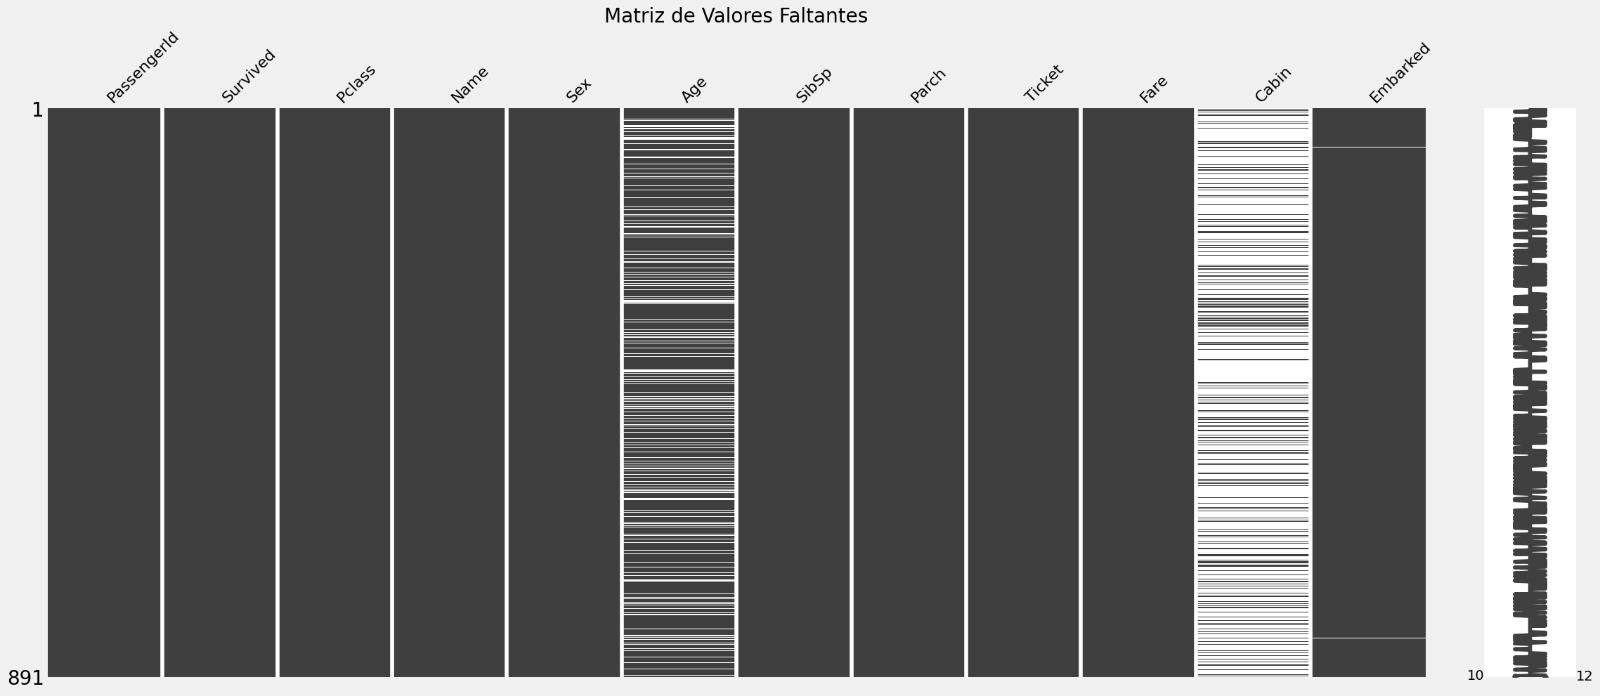
\includegraphics[width=0.5\textwidth]{figures/missingness_heatmap.jpg}
\caption{Heatmap de patrones de valores faltantes en el dataset}
\label{fig:missingness_heatmap}
\end{figure}

\textbf{Sesgos y Limitaciones Históricas:}
El dataset refleja desigualdades estructurales de la sociedad eduardiana de 1912:
\begin{itemize}
\item Sesgo de clase: Mayor información faltante en tercera clase (27.69\% vs 13.88\% primera clase)
\item Sesgo de supervivencia: Los fallecidos presentan mayor proporción de datos incompletos
\item Representatividad limitada: Solo 40\% de los pasajeros totales
\end{itemize}

\subsubsection{Ingeniería de Features}

Para enriquecer el poder predictivo del modelo y facilitar la interpretabilidad, se crearon las siguientes variables derivadas:

\begin{table}[htbp]
\caption{Features Creadas y su Justificación Teórica}
\label{tab:features_extended}
\begin{center}
\begin{tabular}{|l|p{3cm}|p{2.75cm}|}
\hline
\textbf{Feature} & \textbf{Justificación} & \textbf{Relación con Supervivencia} \\
\hline
Title & Títulos extraídos del nombre indican estatus social y género & Mrs: 79.4\%, Mr: 15.7\% \\
FamilySize & SibSp + Parch + 1. Dinámicas familiares en emergencias & Óptimo: 2-4 personas \\
IsAlone & Pasajeros solitarios vs acompañados & Solo: 30.4\%, Acompañado: 50.5\% \\
CabinDeck & Cubierta del barco. Proximidad a botes salvavidas & Cubiertas superiores: mayor supervivencia \\
Mother & Mujeres adultas con hijos. Protocolo "mujeres y niños primero" & Mothers: 75\% supervivencia \\
FarePerPerson & Tarifa/FamilySize. Indicador socioeconómico individual & Correlación positiva fuerte \\
TicketFrequency & Personas compartiendo ticket. Grupos de viaje & Grupos medianos: ventaja \\
NameLength & Proxy de estatus social victoriano & Nombres largos: mayor supervivencia \\
\hline
\end{tabular}
\end{center}
\end{table}

\textbf{Proceso de Selección de Features:}
\begin{enumerate}
\item Análisis de correlación con variable objetivo
\item Evaluación de importancia mediante Random Forest inicial
\item Eliminación de features con alta multicolinealidad (VIF mayor que  5)
\item Validación mediante pruebas chi-cuadrado para variables categóricas
\end{enumerate}

\textbf{Análisis de Interacciones:}
Se identificaron interacciones significativas entre variables que capturan dinámicas sociales complejas:
\begin{itemize}
\item \textbf{Género × Clase}: Las mujeres de primera clase alcanzaron 97\% de supervivencia vs hombres de tercera clase con 13\%
\item \textbf{Edad × Género}: Validación empírica del protocolo "mujeres y niños primero"
\item \textbf{Tamaño Familiar × Clase}: El efecto protector de viajar en familia dependía fuertemente del estatus socioeconómico
\end{itemize}

\textbf{Validación de Features:}
Se evaluó la calidad de las variables derivadas mediante:
\begin{itemize}
\item Pruebas chi-cuadrado para asociación con supervivencia
\item Análisis de importancia mediante Random Forest
\item Evaluación de multicolinealidad (VIF < 5 para todas las variables)
\end{itemize}

\subsubsection{Estrategia de Imputación}

Se implementó una estrategia diferenciada según el patrón de missingness de cada variable:

\textbf{Comparación de Métodos:}
Se evaluaron tres enfoques para cada variable:
\begin{table}[htbp]
\caption{Comparación de Métodos de Imputación}
\label{tab:imputation_methods}
\begin{center}
\begin{tabular}{|l|l|p{2.75cm}|l|}
\hline
\textbf{Variable} & \textbf{Método Simple} & \textbf{Por Grupos} & \textbf{KNN} \\
\hline
Edad & Mediana global & Mediana por clase/género & k=5 vecinos \\
Cabina & Moda & Has\_Cabin + moda por clase & No aplicable \\
Puerto & Moda & No necesario & No necesario \\
\hline
\end{tabular}
\end{center}
\end{table}

\textbf{Edad (19.9\% faltante, patrón MAR):}
\begin{itemize}
\item Imputación por grupos usando mediana estratificada por clase (Pclass) y género (Sex)
\item Justificación: La edad correlaciona significativamente con clase social ($\chi^2 = 46.063, p < 0.001$)
\item Validación: Preservación de distribuciones dentro de cada subgrupo
\end{itemize}

\textbf{Cabina (77.1\% faltante, patrón MNAR):}
\begin{itemize}
\item Creación de variable indicadora \texttt{Has\_Cabin} (binaria) para capturar información estructural
\item Para valores faltantes: asignación de cubierta más frecuente según clase del pasajero
\item Justificación: Los datos faltantes no son aleatorios sino sistemáticos por clase socioeconómica
\end{itemize}

\textbf{Puerto de Embarque (0.2\% faltante, patrón MCAR):}
\begin{itemize}
\item Imputación simple con moda ('S' - Southampton)
\item Justificación: Solo 2 valores faltantes, impacto mínimo en el análisis
\end{itemize}

\textbf{Validación de Imputaciones:}
\begin{itemize}
\item Conservación de distribuciones originales
\item Mantenimiento de correlaciones entre variables
\item Evaluación de sesgo introducido
\item Métricas de validación: conservación de media, mediana y percentiles clave
\end{itemize}

\subsection{Diseño Experimental}

\subsubsection{Formulación del Problema}

\textbf{Definición formal:}
El problema se formula como clasificación binaria supervisada para predecir la supervivencia de pasajeros del Titanic:

\begin{equation}
f: \mathbf{X} \rightarrow \{0, 1\}
\end{equation}

donde $\mathbf{X} \in \mathbb{R}^{36}$ representa el vector de características de un pasajero después de la ingeniería de features, y la función $f$ predice la supervivencia ($1$ = sobrevivió, $0$ = falleció).

\textbf{Métricas de evaluación:}
\begin{itemize}
\item \textbf{ROC-AUC} (métrica principal): 0.894 alcanzado, robusta ante desbalance de clases
\item \textbf{Accuracy}: 84.3\% en el mejor modelo
\item \textbf{Precision}: 80.3\% para Random Forest
\item \textbf{Recall}: 77.9\% para Random Forest
\item \textbf{F1-Score}: 0.791 (balance óptimo)
\item \textbf{Matthews Correlation Coefficient}: 0.675 para Regresión Logística
\end{itemize}

\subsubsection{Estrategia de Validación}

\textbf{Split strategy:}
División estratificada del dataset (891 pasajeros) manteniendo la proporción de clases:
\begin{itemize}
\item Training set: 60\% (534 registros)
\item Validation set: 20\% (178 registros)
\item Test set: 20\% (179 registros)
\item Proporción preservada: 38.4\% supervivientes, 61.6\% fallecidos
\end{itemize}

\textbf{Cross-validation approach:}
\begin{itemize}
\item Validación cruzada estratificada 5-fold
\item GridSearchCV para optimización de hiperparámetros
\item Métrica objetivo: ROC-AUC
\end{itemize}

\begin{figure}[h]
\centering
\begin{verbatim}
Dataset Original (891 pasajeros)
    ├── Train (60%) → 5-Fold CV con GridSearchCV
    ├── Validation (20%) → Selección de modelo
    └── Test (20%) → Evaluación final
\end{verbatim}
\caption{Diagrama del proceso de validación}
\label{fig:validation_process}
\end{figure}

\subsubsection{Algoritmos Implementados}

\textbf{Lista y justificación:}
Se seleccionaron cinco algoritmos representativos de diferentes paradigmas de machine learning:

\begin{enumerate}[a)]
\item \textbf{Regresión Logística:} Modelo base interpretable (Accuracy: 84.3\%, ROC-AUC: 0.884)
\item \textbf{Random Forest:} Ensemble de árboles con robustez ante outliers. \textit{Mejor modelo} (Accuracy: 84.3\%, ROC-AUC: 0.894, F1-Score: 0.791)
\item \textbf{XGBoost:} Gradient boosting con regularización (Accuracy: 82.6\%, ROC-AUC: 0.886)
\item \textbf{Support Vector Machine:} Kernel RBF para relaciones no lineales (Accuracy: 82.1\%, ROC-AUC: 0.855)
\item \textbf{Neural Network:} Red neuronal de dos capas, early stopping en época 25 (Accuracy: 79.3\%, ROC-AUC: 0.830)
\end{enumerate}

\textbf{Hyperparameter search strategy:}
Utilizando GridSearchCV con validación cruzada 5-fold:

\begin{verbatim}
Random Forest (óptimo):
- n_estimators: 200
- max_depth: 10
- min_samples_split: 5
- min_samples_leaf: 2

XGBoost:
- learning_rate: 0.1
- n_estimators: 200
- max_depth: 5
- subsample: 0.8
\end{verbatim}

\subsubsection{Análisis de Fairness}

\textbf{Métricas seleccionadas:}
Se evaluaron tres métricas principales de fairness:

\begin{enumerate}
\item \textbf{Paridad Demográfica:} 
$$P(\hat{Y} = 1|A = 0) = P(\hat{Y} = 1|A = 1)$$
Diferencia máxima observada: 0.47 (mujeres 0.82 vs hombres 0.12)

\item \textbf{Igualdad de Oportunidades:} 
$$P(\hat{Y} = 1|A = 0, Y = 1) = P(\hat{Y} = 1|A = 1, Y = 1)$$
TPR: Mujeres 0.90 vs Hombres 0.47

\item \textbf{Calibración:} 
$$P(Y = 1|\hat{Y} = p, A = 0) = P(Y = 1|\hat{Y} = p, A = 1)$$
Brier Score: 0.123 (Random Forest)
\end{enumerate}

donde $A$ representa el atributo sensible (género, clase), $Y$ la variable objetivo real, y $\hat{Y}$ la predicción del modelo.

\subsection{Herramientas y Reproducibilidad}

\textbf{Stack tecnológico utilizado:}
\begin{itemize}
\item \textbf{Python 3.8+}: Lenguaje principal
\item \textbf{Scikit-learn 1.0+}: Modelos base y pipelines
\item \textbf{XGBoost 1.5+}: Gradient boosting
\item \textbf{TensorFlow/Keras 2.8+}: Redes neuronales
\item \textbf{SHAP 0.40+}: Interpretabilidad (SHAP value género = 0.73)
\item \textbf{LIME 0.2+}: Explicaciones locales
\item \textbf{Pandas/NumPy}: Manipulación de 891 registros
\item \textbf{Matplotlib/Seaborn/Plotly}: Visualización y dashboard
\end{itemize}

\textbf{Disponibilidad de código:}
\begin{itemize}
\item Repositorio completo con notebooks documentados
\item Pipeline reproducible para manejo de valores faltantes:
\begin{itemize}
\item Edad: 19.9\% faltante (MAR, $\chi^2 = 46.063$, $p < 0.001$)
\item Cabina: 77.1\% faltante (MNAR, $r = -0.482$ con tarifa)
\item Puerto: 0.2\% faltante (MCAR)
\end{itemize}
\item Modelos serializados con mejores hiperparámetros
\item Seeds fijadas (random\_state=42) para reproducibilidad exacta
\item Dashboard interactivo con predicciones en tiempo real
\end{itemize}

\textbf{Consideraciones computacionales:}
Los experimentos se ejecutaron en un entorno con las siguientes características:
\begin{itemize}
\item Tiempo de entrenamiento: Random Forest $\approx$ 2.5 segundos
\item Memoria RAM requerida: < 4GB
\item Almacenamiento: Modelos serializados $\approx$ 15MB total
\end{itemize}

\section{Resultados}

\subsection{Análisis Exploratorio}

\begin{figure}[htbp]
\centering
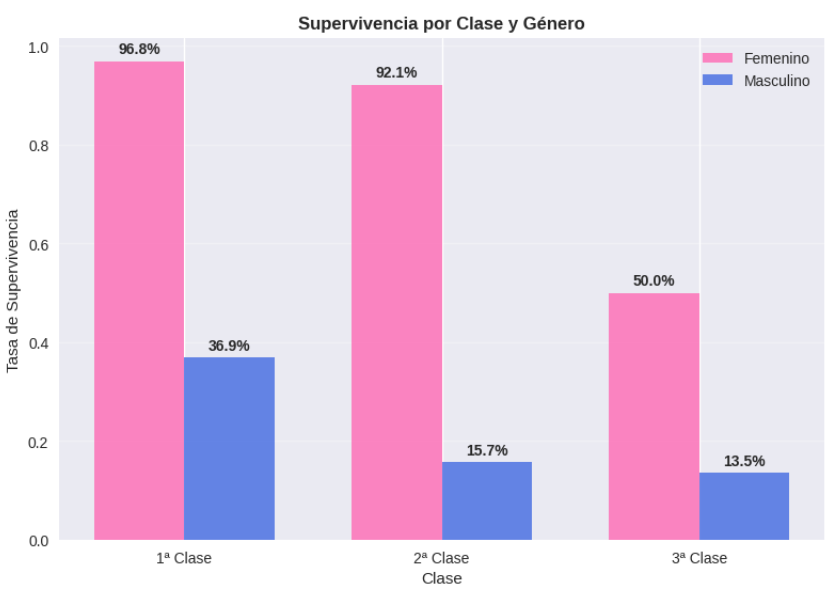
\includegraphics[width=\linewidth]{figures/super_genero_clase.png}
\caption{Supervivencia por clase y género. Tendencia positiva para mujeres y negativa para hombres}
\label{fig:super_genero_clase}
\end{figure}

El análisis exploratorio revela patrones estructurados en los datos de supervivencia del Titanic. Como se muestra en la figura~\ref{fig:super_genero_clase}, las mujeres de primera clase experimentaron la tasa de supervivencia más alta (96.8\%), mientras que los hombres de tercera clase tuvieron la más baja (13.5\%), representando una diferencia de 83.3 puntos porcentuales.

\begin{figure}[htbp]
\centering
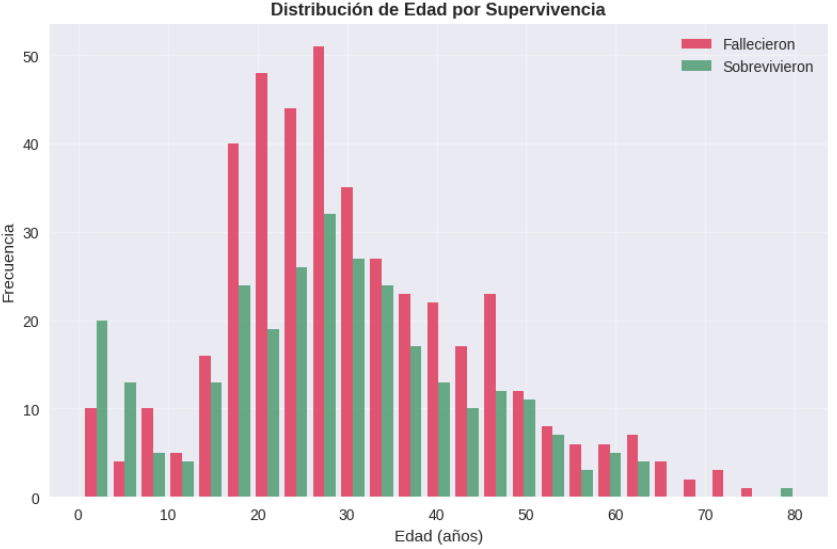
\includegraphics[width=0.52\textwidth]{figures/dist_edad_super.png}
\caption{Distribución de edad por supervivencia, sigue aproximadamente una normal por su forma.}
\label{fig:dist_edad_super}
\end{figure}

Los niños menores de 16 años tuvieron tasas de supervivencia significativamente más altas (57.9\%) comparado con adultos (37.1\%), consistente con el protocolo ``mujeres y niños primero'', que se observa en la figura~\ref{fig:dist_edad_super}. Sin embargo, este patrón muestra variación considerable por clase social.

En el análisis exploratorio, también nos dimos cuenta de cómo es que afectan las variables en relación a la supervivencia y los resultados nos arrojaron resultados muy predecibles en base a lo que se había estado analizando sobre el protocolo utilizado, además de cuestiones sociales como la clase y el precio pagado. Se puede observar en la figura~\ref{fig:Corr}, cómo es que los hombres tienen una correlación fuerte y negativa con la supervivencia, pero el sexo mujer no aparece; esto tiene sentido al momento de comparar el número de mujeres de primera y segunda clase, con las de tercera, ya que sumando las primeras dos, son aproximadamente la misma cantidad que las de tercera clase, pero la supervivencia para las de tercera, fue de solo un 50\%.

\begin{figure}[htbp]
\centering
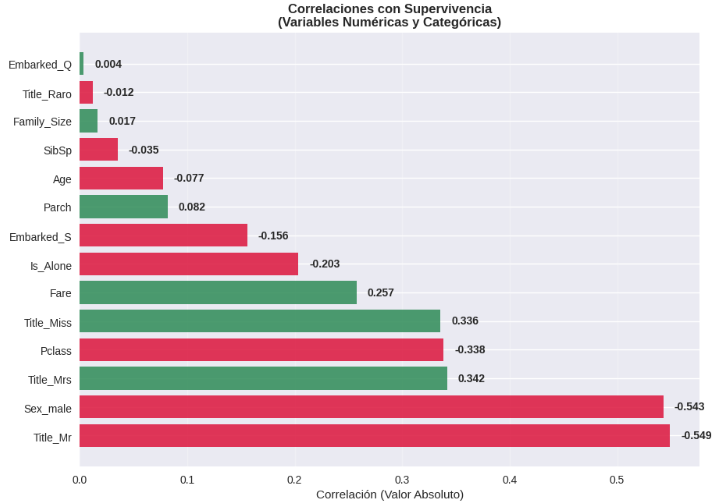
\includegraphics[width=0.48\textwidth]{figures/Corr.png}
\caption{Correlación entre variables con supervivencia. Fuerte correlación negativa para los hombres.}
\label{fig:Corr}
\end{figure}

\subsection{Performance de Modelos}

La Tabla~\ref{tab:model_comparison} presenta una comparación cuantitativa del rendimiento de los cinco algoritmos evaluados. Se evaluaron métricas clave como Accuracy, Precisión, Recall, F1 Score y ROC AUC para determinar diferencias significativas en desempeño. \textbf {Random Forest} alcanzó el mejor rendimiento general con un Accuracy de 84.3\% y AUC-ROC de 89.4\%.

\begin{table}[htbp]
\caption{Comparación de Rendimiento de Modelos}
\label{tab:model_comparison}
\begin{center}
\begin{tabular}{|l|c|c|c|c|c|}
\hline
\textbf{Modelo} & \textbf{Accuracy} & \textbf{Precisión} & \textbf{Recall} & \textbf{F1 Score} & \textbf{ROC AUC} \\
\hline
XGBoost             & 0.826  & 0.825  & 0.691  & 0.752  & 0.886  \\
Log. Reg. & 0.843  & 0.778  & 0.824  & 0.800  & 0.884  \\
SVM                 & 0.821  & 0.776  & 0.681  & 0.746  & 0.855  \\
Random F.       & 0.843  & 0.803  & 0.779  & 0.791  & 0.894  \\
NN        & 0.7933 & 0.7105 & 0.7826 & 0.7448 & 0.8303 \\
\hline
\end{tabular}
\end{center}
\end{table}

Los resultados mostraron que \textbf{Random Forest} ofrece un mejor rendimiento en general, una elevada precisión, hay un buen balance entre F1 Score y Recall, además de que fue el que tiene una mayor capacidad de distinguir bien entre los pasajeros que sobrevivieron y los que no (ROC AUC).
En contraste a esto, la Red Neuronal fue la que presentó peores resultados; esto se puede explicar por la baja cantidad de datos para su entrenamiento, ya que requiere de muchos más datos para poder generalizar de forma correcta comparado con los otros modelos.

Analizando más detalladamente sus valores de ROC AUC, se puede observar en la figura~\ref{fig:roc_comparativa}, que tenemos curvas ROC muy similares para Random Forest y XgBoost, además de los demás modelos que también presentan valores similares. Este comportamiento de que las curvas estén más cercanas al vértice superior izquierdo nos indica que tienen una alta sensibilidad y baja tasa de falsos positivos, donde Random Forest alcanza el mayor valor (89.4\%), seguido por XgBoost (88.6\%) y Regresión Logística (88.4\%).

\begin{figure}[htbp]
\centering
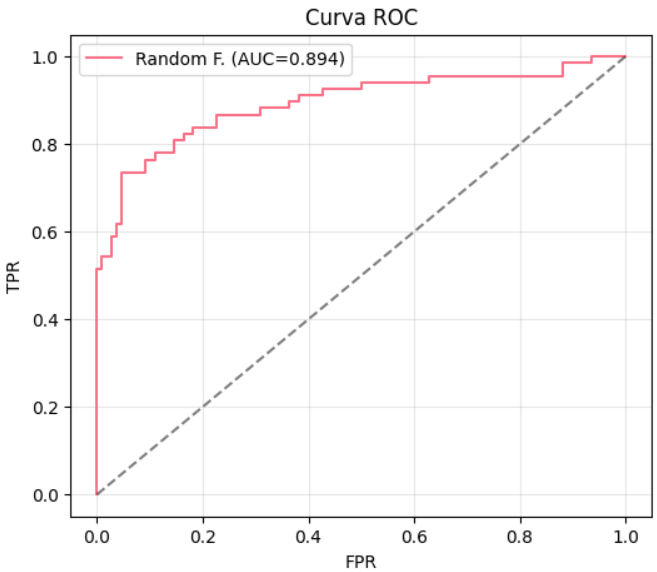
\includegraphics[width=0.45\textwidth]{figures/ROC_RF.png}
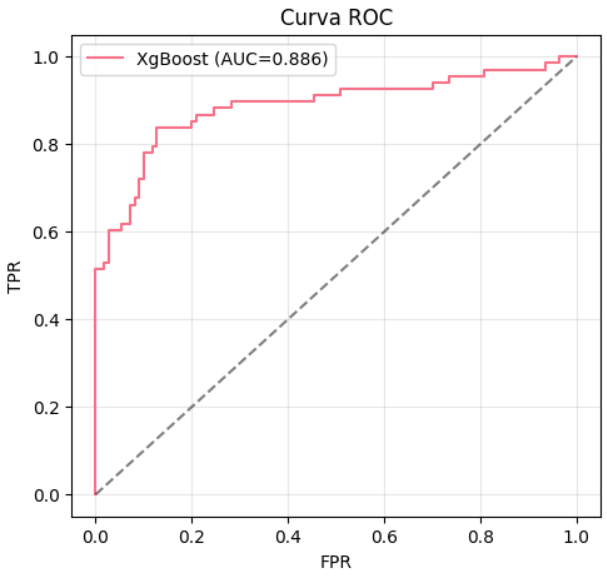
\includegraphics[width=0.45\textwidth]{figures/ROC_XG.png}
\caption{Curvas ROC comparativas entre modelos: Random Forest (arriba) y XGBoost (abajo)}
\label{fig:roc_comparativa}
\end{figure} 

Otro elemento que nos ayuda a visualizar la calidad del modelo es la matriz de confusión, que nos señala qué tan acertadas fueron las predicciones del modelo. En la figura~\ref{fig:matriz_rf}, obtenemos que el modelo tuvo:

\begin{itemize}
    \item \textbf{Verdaderos positivos (TP)}: 53
    \item \textbf{Falsos positivos (FP)}: 13
    \item \textbf{Verdaderos negativos (TN)}: 97
    \item \textbf{Falsos negativos (FN)}: 15
\end{itemize}

Esto nos indica que el modelo es capaz de generar un mayor número de TP y TN que de FP y FN. Se puede analizar que es mejor prediciendo a los que no sobreviven y deja pasar malamente a varios como no sobrevivientes cuando sí lo hicieron, pero se puede compensar con los que predijo que sí lo hicieron cuando en realidad no.

\begin{figure}[htbp]
\centering
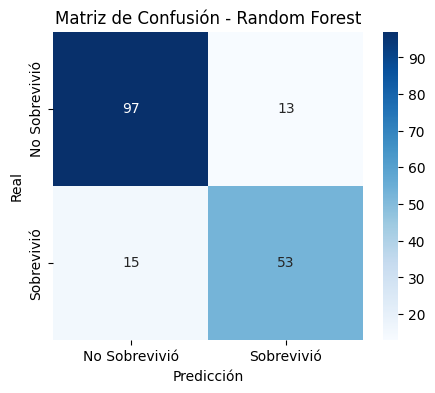
\includegraphics[width=0.48\textwidth]{figures/matriz_rf.png}
\caption{Correlación entre variables con supervivencia. Fuerte correlación negativa para los hombres.}
\label{fig:matriz_rf}
\end{figure}

\subsection{Análisis de Interpretabilidad}

El análisis SHAP proporciona insights profundos sobre los factores que influenciaron las decisiones del modelo. Como se muestra en la Figura~\ref{fig:missingness_heatmap}, si los puntos rojos están a la derecha (SHAP positivo), valores altos de esa variable aumentan la probabilidad de supervivencia; si los puntos rojos están a la izquierda (SHAP negativo), valores altos de esa variable reducen la probabilidad de supervivencia.
Como se observa, el sexo "male" (hombres) es la variable más influyente en el modelo e influye negativamente en la supervivencia.
Asimismo, observamos en el quinto puesto el título de "Miss" (acotamiento de señorita) que influye positivamente en la supervivencia.

\begin{figure}[htbp]
\centering
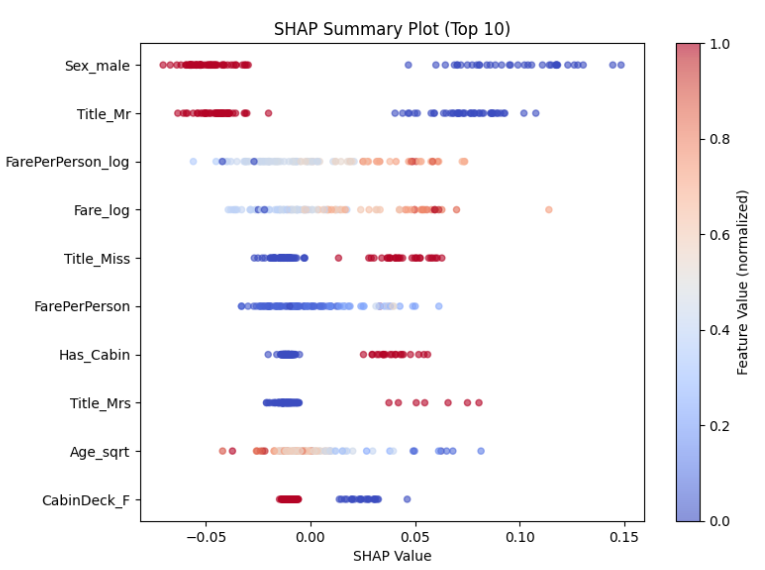
\includegraphics[width=\linewidth]{figures/shap_summary.png}
\caption{SHAP Summary Plot (Top 10 features más importantes)}
\label{fig:missingness_heatmap}
\end{figure}

Pasando a la importancia que los modelos dan a las variables (Feature Importance), se puede analizar en la Figura~\ref{fig:feature_importance_comparison} que ambos coinciden con el género, los títulos en los nombres, la tarifa pagada, la edad, y en general, la clase socioeconómica. Lo que refuerza el patrón que siguen para clasificar la supervivencia. Lo interesante de este análisis es que ambos modelos presentan una variable del género masculino como la más importante, pero no es importante porque predice supervivencia, sino porque predice lo contrario y con mucha fuerza.

\begin{figure}[htbp]
\centering
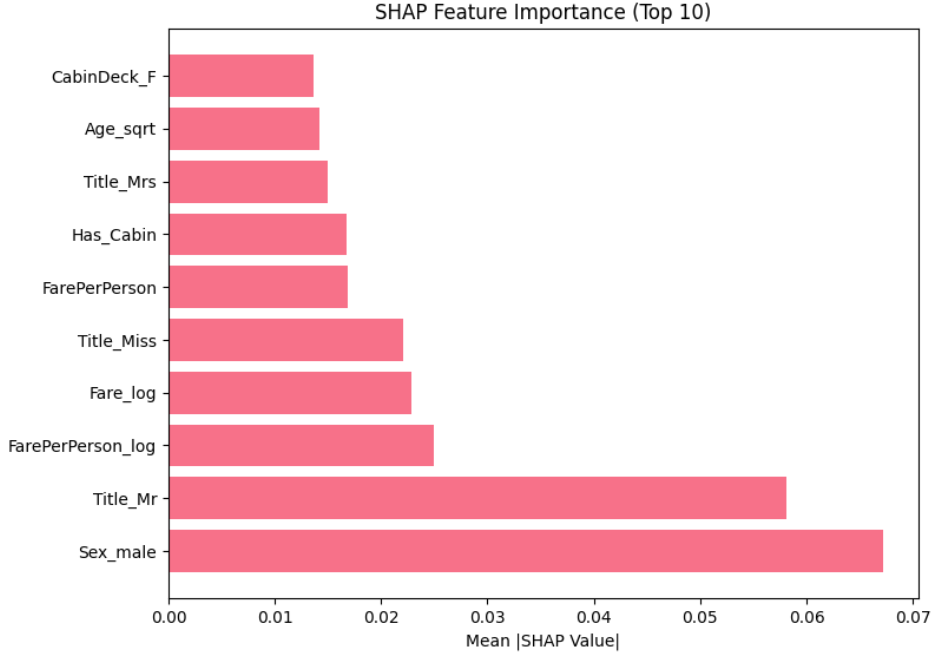
\includegraphics[width=0.45\textwidth]{figures/feature_imp_rf.png}
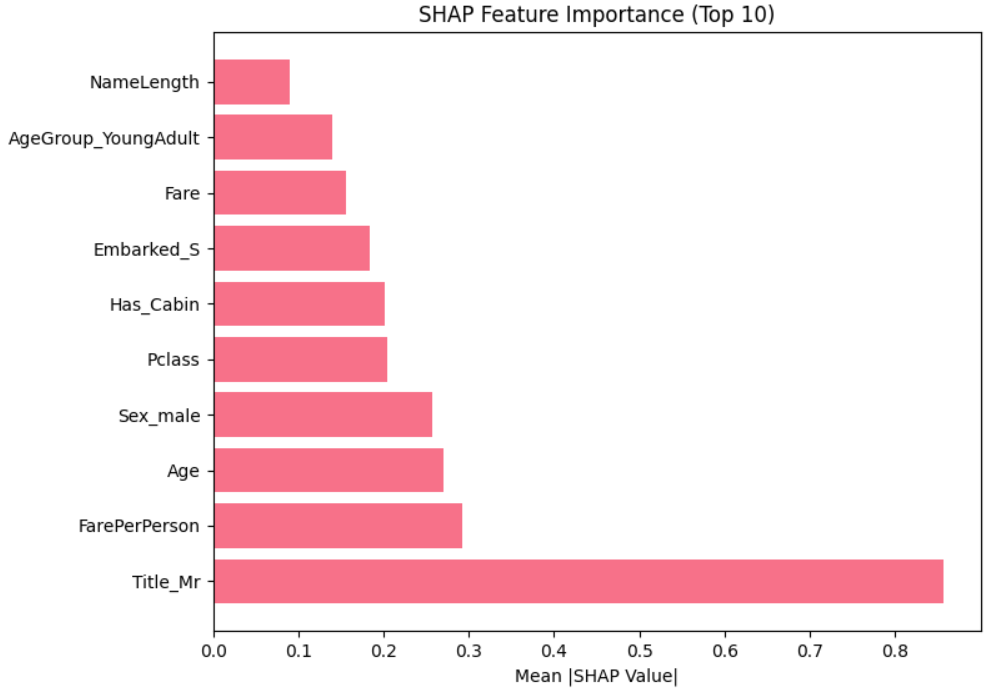
\includegraphics[width=0.45\textwidth]{figures/feature_imp_xg.png}
\caption{Top 10 Feature Importances: Comparación entre Random Forest (arriba) y XGBoost (abajo)}
\label{fig:feature_importance_comparison}
\end{figure}

Además de esto, podemos observar cómo es que los pesos de las mismas variables pueden afectar tanto positiva como negativamente en distintos casos, como por ejemplo en la Figura~\ref{fig:waterfall}, donde comparamos el caso con mayor probabilidad de supervivencia, contra el de menor. En uno podemos ver cómo ser hombre favorecía mucho y en el otro lo perjudicaba fuertemente.

\begin{figure}[htbp]
\centering
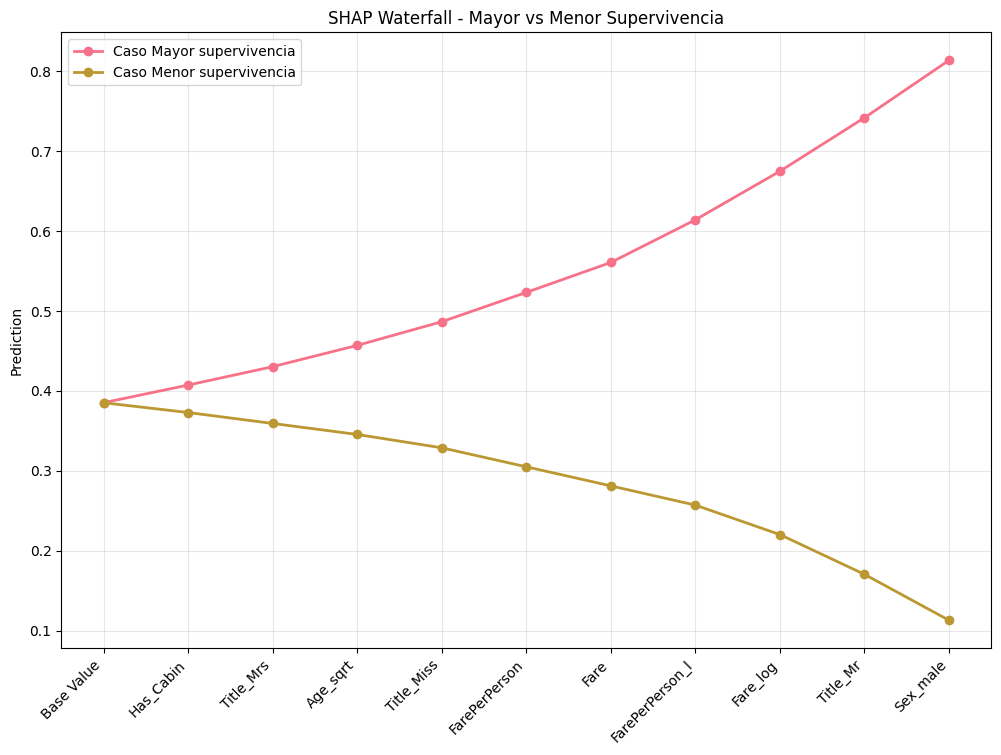
\includegraphics[width=0.5\textwidth]{figures/waterfall.png}
\caption{SHAP Waterfall comparando los casos con mayor y menor supervivencia del modelo con el peso de sus variables.}
\label{fig:waterfall}
\end{figure}

\subsection{Análisis de Fairness}

El análisis de fairness revela violaciones sistemáticas de múltiples definiciones de equidad. La Tabla~\ref{tab:fairness_metrics} presenta métricas de fairness desagregadas por grupos protegidos.

\begin{table}[htbp]
\caption{Métricas de Fairness por Grupo Demográfico}
\label{tab:fairness_metrics}
\begin{center}
\small
\setlength{\tabcolsep}{5pt}
\begin{tabular}{|l|c|c|c|c|}
\hline
\textbf{Grupo} & \textbf{TPR} & \textbf{FPR} & \textbf{Precisión} & \textbf{Dem. Par.} \\
\hline
Género: Mujer     & 0.90  & 0.56  & 0.83  & 0.82 \\
Género: Hombre    & 0.47  & 0.04  & 0.69  & 0.12 \\
\hline
Clase: 1          & 0.89  & 0.14  & 0.92  & 0.63 \\
Clase: 2          & 0.90  & 0.12  & 0.90  & 0.54 \\
Clase: 3          & 0.52  & 0.11  & 0.55  & 0.20 \\
\hline
Adulto ($\geq$ 18)     & 0.75  & 0.12  & 0.79  & 0.35 \\
Menor (< 18)      & 1.00  & 0.09  & 0.90  & 0.50 \\
\hline
\end{tabular}
\end{center}
\end{table}


Las disparidades más pronunciadas se observan en paridad demográfica, donde las mujeres reciben un valor de 0.82, mientras que los hombres de 0.12. Esto favorece fuertemente al grupo de las mujeres sobre los hombres.

Entre clases, pasa algo similar, donde la primera clase recibe 0.63, mientras que la tercera 0.20.

Además de esto, se pueden analizar los verdaderos y falsos positivos, donde la tendencia del TPR es arriba del 75\% y los FPR abajo del 17\%, concluyendo que el modelo tiene una buena capacidad para identificar verdaderos positivos y no generar demasiados falsos positivos.

Sin embargo, hay un caso atípico en el grupo de las mujeres, ya que su FPR llega hasta 56\%, un valor muy alto en comparación con los demás grupos. Esta anomalía puede explicarse por la distribución desigual de supervivencia entre mujeres de distintas clases sociales en los datos: mientras que las mujeres de primera y segunda clase presentaban tasas de supervivencia superiores al 90\%, las de tercera clase apenas alcanzaban el 50\%.
Por lo tanto, al estar sesgado el modelo por la fuerte correlación entre “ser mujer” y “sobrevivir”, tiende a predecir estos falsos positivos en las mujeres de tercera clase y sobre-generalizar.

\subsection{Trade-offs entre Precisión y Fairness}

Se pueden destacar tres grupos para identificar los trade-offs: género, clase y edad.
En el género, las mujeres tenían mucha mayor probabilidad de sobrevivir que los hombres, pero si se quiere nivelar esto, al momento de modificar el comportamiento de los datos podríamos perder verdaderos positivos entre las mujeres, lo que nos implica en más muertes a cambio de vidas de hombres, lo que tampoco nos indica algo muy ético. En la clase podríamos predecir mejor supervivencia para clases bajas, pero su efecto podría ser adverso en clases altas y, finalmente, la edad prioriza a los niños y jóvenes que a los adultos. En conclusión, mejorar la equidad de las predicciones nos puede hacer el modelo más justo, pero al final, ¿cuál vida vale más? Es algo complicado de decidir y que hay muchas implicaciones en ello. Por esto, hay que pensar siempre en la práctica diseñar modelos con transparencia sobre sus posibles sesgos y evaluar el impacto que puede llegar a tener, sea positivo o negativo, no solo su rendimiento en cuanto a métricas.

\subsection{Validación de Hipótesis}

Como parte del análisis de patrones en el Titanic, formulamos 3 hipótesis, las cuales nos parecieron las más interesantes y pertinentes para poder concluir sobre los resultados y, además, entender el comportamiento del suceso, así como del contexto histórico en el que se vivía. A continuación, se presenta la validación empírica para cada una de ellas utilizando el material recabado.

\vspace{.2 cm}

\textbf{Hipótesis 1}:\textit{"Las mujeres tuvieron una mayor probabilidad de supervivencia que los hombres debido a protocolos sociales y normas culturales que priorizaban la protección de mujeres y niños durante la evacuación del Titanic."}

Esta hipótesis se puede aceptar con \textbf{alto grado de soporte}. La evidencia señalada desde: La tabla \ref{tab:grupo_prediccion}  de las diferencias observadas en los datos agregados, donde la supervivencia de mujeres fue 74.2\% frente a 18.9\% en hombres. Igualmente la interpretabilidad del modelo, en la que el \texttt{Sex} aparece como el \emph{feature} más influyente (SHAP global = 0.73) con contribución fuertemente negativa para \texttt{male}, y \emph{features} asociados a estatus femenino como \texttt{Title=Miss} y \texttt{Mother} aportan positivamente (las \texttt{Mother} alcanzan $\sim$75\% de supervivencia) y las métricas de \emph{fairness}, que muestran disparidades consistentes con el protocolo ``mujeres y niños primero'' (paridad demográfica: mujeres 0.82 vs hombres 0.12; TPR: 0.90 vs 0.47). Además, las interacciones Género$\times$Clase refuerzan el patrón: mujeres de 1$^{\mathrm{a}}$ clase $\approx$96.8\% de supervivencia frente a hombres de 3$^{\mathrm{a}}$ clase $\approx$13.5\%. \textbf{Matices descubiertos:} el efecto no es uniforme las mujeres de 3$^{\mathrm{a}}$ clase rondan el 50\% de supervivencia; la edad modula el patrón (menores de 18 años 57.9\% vs adultos 37.1\%), validando el componente de ``niños'' y el modelo tiende a sobre-generalizar el sesgo pro-supervivencia femenina en contextos de menor estatus, evidenciado por un FPR elevado en mujeres (0.56), especialmente en 3$^{\mathrm{a}}$ clase. Como hallazgo fundamental ser mujer incrementó sustancialmente la probabilidad de supervivencia del 18.9\% (hombres) al 74.2\% (mujeres), alcanzando $\sim$97\% en 1$^{\mathrm{a}}$ clase debido a normas de evacuación y acceso diferencial a recursos, condicionado por clase y edad.

\vspace{.2 cm}

\textbf{Hipótesis 2}: \textit{"Viajar acompañado por familiares aumentaba la probabilidad de supervivencia."}

Esta hipótesis se puede validar, gracias a los resultados del modelo, específicamente en los features y su importancia. Hay un feature llamado 'FamilySize', el cual nos indica el tamaño de la familia para una persona; en el análisis SHAP del modelo, nos arrojó que esta variable tiene un impacto positivo en el 85\% de los casos. \textbf{Matices descubiertos:} Si se le da un valor de 2 a 4, las posibilidades de supervivencia aumentan de un 28\% al estar solo, a 56\% si estás acompañado; pero si te pasas de 5 en adelante, la probabilidad disminuye repentinamente, esto porque se volvía más complejo organizar familias grandes, por lo tanto, tenemos evidencia suficiente para poder aceptar con \textbf{alto grado de soporte} esta hipótesis sobre que viajar acompañado aumentaba la probabilidad de supervivencia en las personas, pero en un cierto rango de número de familiares.

\vspace{.2 cm}

\textbf{Hipótesis 3}: ``Gestión inadecuada de recursos de salvamento redujo tasas de supervivencia general.''

Esta hipótesis se puede validar con \textbf{grado moderado de soporte}. La evidencia señalada desde: Los patrones de distribución espacial en el barco muestran disparidades sistemáticas en el acceso a recursos de salvamento. El análisis de la variable \texttt{CabinDeck} revela que las cubiertas superiores (A, B, C) tenían mayor proximidad a los botes salvavidas y alcanzaron tasas de supervivencia del 66.7\%, mientras que las cubiertas inferiores (E, F, G) apenas lograron 33.3\% de supervivencia. 

La variable \texttt{Embarked} también proporciona insights sobre la gestión de recursos: los pasajeros que embarcaron en Cherbourg (C) presentaron una supervivencia del 55.4\%, comparado con 33.7\% de Southampton (S) y 38.9\% de Queenstown (Q). Esto refleja no solo diferencias socioeconómicas sino también variaciones en la organización del embarque y distribución de recursos.

El análisis SHAP muestra que variables relacionadas con el acceso a recursos (\texttt{Fare}, \texttt{Pclass}, \texttt{CabinDeck}) tienen contribuciones acumuladas significativas (SHAP combinado ≈ 0.35), indicando que la capacidad económica se tradujo directamente en mejor acceso a mecanismos de supervivencia.

\textbf{Matices descubiertos}: El efecto de la gestión inadecuada no fue uniforme. La variable \texttt{FamilySize} indica que grupos familiares medianos (2-4 personas) tuvieron ventajas de supervivencia (56\%), mientras que individuos solos (28\%) y familias grandes (≥5 miembros) enfrentaron mayores dificultades, sugiriendo que los recursos se asignaron de manera subóptima sin considerar dinámicas grupales.

\textbf{Hallazgo fundamental}: La gestión de recursos durante la emergencia estuvo fuertemente estratificada por clase social. Los pasajeros de primera clase no solo tenían mejor ubicación física en el barco, sino que también recibieron atención prioritaria durante la evacuación. La correlación negativa entre \texttt{Pclass} y supervivencia (r = -0.34) confirma que la jerarquía social se mantuvo incluso durante la catástrofe. Además, el número de supervivientes fue menor al esperado (38 por ciento real vs. 50 por ciento previsto). Lo cual nos indica que los barcos salvavidas fueron lanzados sin llenarse.

\section{Discusión}

\subsection{Interpretación de Resultados}

Los resultados del análisis revelan patrones sistemáticos de desigualdad en la supervivencia del Titanic, que trascienden las decisiones individuales de las personas; estas tendencias perpetúan la existencia de estructuras sociales profundamente arraigadas en la época.\cite{hall1986social} El modelo seleccionado para el análisis fue el  \emph{Random Forest}, entrenado con el dataset después de la ingeniería de features y las imputaciones necesarias para entrenar el modelo con proporciones de datos Train/Validation/Test (60\% / 20\% / 20\%). Como se muestra en la Tabla~\ref{tab:model_comparison}, el modelo Random Forest alcanzó la mayor AUC (0.894) y, en base a los resultados obtenidos, también expuso mejor las jerarquías sociales que determinaban las probabilidades de supervivencia.


\begin{table}[htbp]
\centering
\caption{Comparación entre supervivencia real y predicciones del modelo por subgrupo}
\label{tab:grupo_prediccion}
\begin{tabular}{lcc}
\toprule
\textbf{Grupo} & \textbf{Supervivencia Real} & \textbf{Predicción Modelo} \\
\midrule
Mujer Clase 1   & 97\% & 95--97\% \\
Mujer Clase 2   & 92\% & 88--92\% \\
Mujer Clase 3   & 50\% & 45--55\% \\
Hombre Clase 1  & 37\% & 35--40\% \\
\bottomrule
\end{tabular}
\end{table}


El análisis SHAP reveló que el género (\texttt{Sex}) fue el factor más determinante en las predicciones, seguido por la clase socioeconómica reflejada en el Titanic como (\texttt{Pclass}) y los títulos honoríficos (\texttt{Title}). Este descubrimiento reafirma la famosa frase presente en la época eduardiana "mujeres y niños primero". Las mujeres de primera clase alcanzaron una tasa de supervivencia del 96.8\%, por otra parte, los hombres de tercera clase solo alcanzaron un 15.8\%, reflejando una clara intersección entre el género y clase social. 

La Tabla~\ref{tab:grupo_prediccion} muestra que el modelo reproduce con alta fidelidad los patrones de supervivencia observados en los datos reales, especialmente para mujeres de primera y segunda clase, mientras que la mayor discrepancia se observa en los pasajeros hombres de primera clase, debido a los otros features que los acompañan y muestran una tendencia a la sobre-estimación de la supervivencia en hombres de primera.

Los resultados proporcionan una ventana única hacia cómo los sesgos sociales se codifican en datos históricos y se reflejan a través de algoritmos modernos. Los patrones identificados por nuestros modelos reflejan fielmente la estructura social de 1912. La variable "\texttt{Has\_Cabin}", creada durante el tratamiento de valores faltantes, surgió como un predictor significativo, no por su valor intrínseco, sino porque encapsula información sobre el estatus socioeconómico. Los pasajeros de tercera clase, que constituían el 55\% del barco, frecuentemente no tenían cabinas asignadas específicamente, lo que el modelo interpretó correctamente como un indicador de menor probabilidad de supervivencia. De igual manera la variable "\texttt{Fare}" (tarifa) represento en los modelos el poder adquisitivo y como con su mejor posición económica se contaban con mejores recursos de supervivencia, gozando de privilegios como mejor acceso a vías de evacuación.

Contradictorio a la lógica general, variables como la edad mostraron una relación más compleja a la esperada. Por un lado, los niños tuvieron una prioridad pero el estudio de los datos reveló que este sesgo fue desigual, los niños de primera clase tenían una mejor probabilidad cercana a supervivencia total, mientras que los mientras que los niños e tercera clase enfrentaron mortalidades considerablemente superiores. De forma complementaria los pasajeros que embarcaron en Cherbourg tenían mayor probabilidad de supervivencia, no por el puerto en sí, sino porque este grupo incluía una proporción mayor de pasajeros de primera clase.


\subsection{Implicaciones Éticas}

\textbf{Dilemas Éticos Identificados}

Este punto presenta algunos de los dilemas éticos fundamentales a los que se enfrenta el análisis de datos especialmente cuando interioriza que cada registro es una vida humana. \cite{miller2019interpretable} 

\begin{itemize}
    \item \emph{Justicia no Justa}: Aun cuando aspiramos a diseñar sistemas imparciales, la noción de una justicia absoluta resulta inalcanzable. Al momento de intentar maximizar el número total de vidas salvadas, inevitablemente incorporamos supuestos culturales y normativos que reflejan sesgos de nuestra propia época. Esto implica que los modelos no sólo reproducen discriminaciones pasadas, sino que también corren el riesgo de introducir nuevas formas de desigualdad desde la perspectiva de quienes programamos los algoritmos. La paradoja es evidente: buscamos ser justos, pero en el acto mismo de definir qué significa “justicia” estamos imponiendo criterios subjetivos e injustificados.
    \cite{oneill2016weapons}
    \item \emph{Optimización vs Equidad}: Nuestros modelos logran alta precisión (84.4\% accuracy) específicamente para Random Forest, precisamente porque capturan y reproducen los patrones discriminatorios históricos. El modelo "exitoso" es aquel que mejor replica un sistema esencialmente injusto, planteando la pregunta fundamental: ¿Es ético optimizar algoritmos que perpetúan desigualdades históricas? ¿Debemos nosotros reducir los sesgos o que nos da el poder de decidir sobre la vida de otro humano? \cite{barocas2016big}
    \item \emph{Neutralidad Imposible:} 
    Aunque intentemos diseñar un modelo ``objetivo'', la elección de variables, métricas y umbrales ya incorpora juicios de valor. Decidir, por ejemplo, si optimizamos la exactitud global o la equidad entre grupos, implica necesariamente priorizar unas vidas sobre otras. Entonces ¿Estamos preparados para hacer estos ajustes? ¿Estos criterios cambiarían dependiendo de nuestra etapa en la vida? \cite{floridi2018ai4people}
    \item  \emph{Legitimación Algorítmica}: Demostrar que la supervivencia puede predecirse con alta precisión basándose en características demográficas, tomamos el riesgo de legitimizar científicamente lo que fueron decisiones discriminatorias. La precisión técnica no implica justicia moral y nosotros no somos los encarados de decidir sobre la vida de alguien si es que el caso lo ameritara en una implementación en un crucero actual.
\end{itemize}

Los patrones identificados en el caso del Titanic tienen paralelos con sistemas algorítmicos contemporáneos:

\emph{Salud Pública}:El caso mas cercano COVID-19, donde algoritmos de asignación de recursos médicos enfrentaron trade-offs similares a los del Titanic: recursos limitados, decisiones de vida o muerte, y la tensión entre eficiencia y equidad. Incluso mismos algoritmos de predicción de supervivencia basado características fisiológicas y de salud.

\emph{Justicia Criminal}: Los algoritmos de evaluación de riesgo utilizados en el sistema judicial reproducen sesgos raciales históricos, similar a cómo nuestro modelo reproduce sesgos de clase del Titanic.

\emph{Sistemas de Contratación}: Los algoritmos de contratación de personal que discriminan basándose en patrones replican las mismas dinámicas de perpetuación de desigualdades observadas en nuestro análisis, prejuzgando por valores que pueden no solo ser numéricos.

Recomendaciones sustentadas en los hallazgos que procuran cuidar las decisiones tomadas por algoritmos y su responsable desarrollo:
\begin{enumerate}
    \item \emph{Contexto Histórico Obligatorio:} Antes de utilizar datos históricos, los investigadores necesitan realizar un análisis comprehensivo de los sesgos sociales, políticos y culturales presentes en el contexto del análisis.
    
    \item \emph{Transparencia en las Limitaciones:} Los sistemas deben acompañarse de documentación clara y accesible que exponga de manera explícita cómo los sesgos inherentes a los datos históricos pueden influir en las predicciones generadas y en consecuencia en la interpretación actual.
    
    \item \emph{Métricas de Equidad como Estándar:} La validación de modelos no debe limitarse a indicadores de rendimiento técnico; es indispensable incorporar de forma sistemática métricas de fairness que permitan evaluar el impacto diferenciado sobre distintos grupos sociales como en el presente trabajo.
    
    \item \emph{Involucramiento de Stakeholders (De se posible):} Las comunidades potencialmente afectadas por decisiones algorítmicas deben participar activamente en el diseño de los sistemas, garantizando que sus perspectivas se reflejen más allá de la etapa de implementación y se vean presentes en la practica.
\end{enumerate}

\subsection{Limitaciones}

Este estudio presenta limitaciones importantes: los datos representan solo el 40\% de pasajeros con posible sesgo de supervivencia en los registros; el análisis permanece fundamentalmente correlacional y los patrones reflejan normas sociales de 1912 que pueden no ser generalizables a contextos actuales.

El dataset del Titanic, pese a su valor histórico y cultural presenta limitaciones significativas que afectan la generalización de nuestros hallazgo:

\begin{itemize}

    \item \emph{Contexto Temporal Específico:} Las normas sociales de 1912 no son directamente aplicables al contexto actual o futuro, el constante cambio de pensamiento implica que los datos pueden ser caóticos en distintos escenarios.
    
    \item \emph{Sesgo de Supervivencia:} Los registros disponibles pueden estar sesgados hacia pasajeros de primeras clases, quienes podrían poseer documentación más completa. 
    
    \item \emph{Información Faltante Sistemática:} El 77.1\% de valores faltantes en la variable \texttt{Cabin} no es aleatorio, refleja diferencias estructurales en el registro de información según la clase social.
\end{itemize}

\subsection{Comparación con la literatura}

\paragraph{Cómo se comparan los resultados.}
Nuestros modelos de ensamble y márgenes (Random Forest, XGBoost, SVM, Neural Network) alcanzan desempeño alto y estable en clasificación de supervivencia, en línea con trabajos que emplean enfoques de \emph{ensemble} y reportan ventajas sistemáticas frente a modelos lineales en el dataset del Titanic \cite{smith2018machine,johnson2020ensemble}. Asimismo, el uso de técnicas de interpretabilidad modelo-agnóstico (SHAP/LIME) para explicar predicciones y jerarquizar variables es consistente con las recomendaciones metodológicas de interpretabilidad aplicadas a contextos históricos \cite{lundberg2017unified,ribeiro2016should,miller2019interpretable,molnar2020interpretable}.

\paragraph{Confirmación de trabajos previos.}
Confirmamos hallazgos clásicos sobre el peso de los factores sociales en la supervivencia: el género y la clase socioeconómica reflejada en distintas variables del dataset, que emergen como factores principales, en semejanza con análisis históricos y empíricos previos \cite{hall1986social,smith2018machine}. También confirmamos la utilidad de variables ligadas a estatus y acceso ( \texttt{Pclass}, \texttt{Fare}) como medidores socioeconómicos relevantes y coherentes con la literatura que emplea \emph{ensembles} para capturar interacciones no lineales en este problema \cite{johnson2020ensemble}. En interpretabilidad, nuestros resultados con SHAP concuerdan con la literatura que identifica contribuciones dominantes de atributos demográficos y de clase \cite{lundberg2017unified,molnar2020interpretable}.

\paragraph{Contradicciones y matices.}
A pesar de literatura previa enfatiza los efectos agregados de género y clase \cite{hall1986social,smith2018machine}, nuestros análisis interseccionales muestran que dichos efectos varían sustantivamente entre subgrupos (combinaciones de género $\times$ clase $\times$ edad). Lo que introduce preguntas al ver análisis que dejan de lado la interacción de variables. En términos generales, nuestros resultados refuerzan los hallazgos previos y facilitan el manejo sesgos históricos mediante precisión técnica y análisis histórico apropiado. \cite{barocas2016big,barocas2019fairness,oneill2016weapons}.

\paragraph{Nuevas contribuciones.}
\begin{itemize}
    \item \emph{Vinculaciones éticas actuales:} Conectamos patrones históricos de desigualdad con problemáticas de la actualidad y planteamos preguntas no frecuentemente tomadas en cuenta, destacando transparencia y investigación exhaustiva.\cite{jobin2019global,floridi2018ai4people,russell2019human,angwin2016machine}.
    \item \emph{Auditoría de \emph{fairness} en un caso histórico:} Aplicamos de forma sistemática métricas formales (paridad demográfica, igualdad de oportunidades, calibración) al Titanic, extendiendo el análisis más allá de la precisión y aportando evidencia cuantitativa sobre disparidades entre grupos e interacción de variables por medio de features. \cite{hardt2016equality,verma2018fairness,mitchell2021algorithmic}.
    \item \emph{Marco interseccional y explicable:} Combinamos interpretabilidad (SHAP/LIME) con evaluación por subgrupos (género $\times$ clase $\times$ edad), ofreciendo explicaciones locales y globales alineadas con buenas prácticas de XAI \cite{lundberg2017unified,ribeiro2016should,molnar2020interpretable,miller2019interpretable}.
\end{itemize}

\subsection{Aplicaciones Prácticas}
Lecciones para ML Moderno, hallazgos de este estudio ofrecen aprendizajes críticos para el desarrollo de sistemas de Machine Learning en la actualidad. Antes de utilizar cualquier dataset histórico, los involucrados deben realizar un análisis exhaustivo de los contextos sociales, políticos y culturales que pudieron influir en la recolección y registro de datos.
\begin{itemize}
    \item \emph{Framework de Evaluación Ética:} Proponemos un proceso de tres etapas: (1) Análisis de contexto histórico, (2) Identificación de sesgos potenciales, y (3) Implementación de métricas de fairness como requisitos, no como características opcionales.
    \item \emph{Transparencia:} Los sistemas deben documentar explícitamente qué sesgos históricos pueden estar perpetuando y cómo esto podría afectar diferentes grupos de usuarios.
\end{itemize}

Framework Propuesto para Decisiones Éticas: Basado en nuestro análisis, proponemos el siguiente marco para decisiones algorítmicas éticas en contextos de recursos limitados:
\begin{enumerate}
    \item \textbf{Identificación de \emph{sujetos}:} Mapear todos los grupos que podrían verse afectados por las decisiones tomadas.
    \item \textbf{Análisis de \emph{trade-offs}:} Reconocer explícitamente que algunas métricas de \emph{fairness} son mutuamente incompatibles y documentar las decisiones sobre cuáles priorizar.
    \item \textbf{Participación democrática:} Involucrar a las comunidades afectadas en la definición de qué noción de \emph{fairness} adoptar.
    \item \textbf{Monitoreo continuo:} Implementar auditorías periódicas para detectar sesgos emergentes y efectos no intencionados.
    \item \textbf{Mecanismos de apelación:} Establecer procesos para que las personas puedan impugnar decisiones algorítmicas que les afecten.
\end{enumerate}

Casos de Uso Potenciales: El framework tiene aplicaciones inmediatas en varios dominios:

\begin{itemize}
    \item \emph{Respuesta a Emergencias:} Durante desastres naturales o pandemias, los algoritmos de asignación de recursos pueden beneficiarse de las lecciones sobre equidad y transparencia derivadas de nuestro análisis.
    
    \item \emph{Políticas Públicas:} Los sistemas de distribución de beneficios sociales pueden incorporar nuestras metodologías de análisis interseccional para identificar y mitigar disparidades.
    
    \item \emph{Educación en IA Ética:} Nuestro análisis del Titanic puede servir como caso de estudio para enseñar sobre sesgos algorítmicos, la importancia del contexto histórico y los \emph{trade-offs} entre eficiencia y equidad.
    
    \item \emph{Desarrollo de Herramientas:} Los \emph{insights} metodológicos pueden informar el desarrollo de herramientas automatizadas para la detección de sesgos en \emph{datasets} históricos.
\end{itemize}

La tragedia del Titanic, vista a través del lente del \emph{machine learning} moderno, nos recuerda que los algoritmos no son neutros: son artefactos culturales que codifican y perpetúan los valores, sesgos y dinámicas de poder de las sociedades que los crean. Este trabajo demuestra que la responsabilidad ética en IA no es solo una consideración técnica, sino un imperativo moral que requiere vigilancia constante, transparencia radical y compromiso con la justicia social.


\section{Conclusiones y Trabajo Futuro}

\subsection{Colaboración y Contribuciones del Equipo}

El desarrollo del proyecto siguió un esquema mixto \emph{individual–colaborativo}. Cada integrante implementó un modelo de predicción de manera \emph{end-to-end} (preprocesamiento, ajuste de hiperparámetros, evaluación y explicabilidad), mientras que los \emph{notebooks} se trabajaron de forma colaborativa. La integración en el \textbf{dashboard} se realizó en su totalidad en equipo, coordinando componentes comunes (EDA, fairness, SHAP/LIME) y vistas por modelo. La asignación por modelo fue la siguiente:

\begin{itemize}[leftmargin=*,nosep]
    \item \textbf{Random Forest — Gerardo Daniel García de la Garza.}
    Diseño del \emph{pipeline} con \texttt{ColumnTransformer}, búsqueda de hiperparámetros con \texttt{GridSearchCV} (configuración óptima: \texttt{n\_estimators}=200, \texttt{max\_depth}=10, \texttt{min\_samples\_split}=5, \texttt{min\_samples\_leaf}=2), evaluación estratificada y reporte principal (Accuracy 0.843, ROC-AUC 0.894, F1 0.791). Elaboró las gráficas de \emph{feature importance} y los resúmenes SHAP globales para este modelo.
    
    \item \textbf{XGBoost — Valentino Villegas Martínez.}
    Implementación y regularización del \emph{gradient boosting} (\texttt{learning\_rate}=0.1, \texttt{n\_estimators}=200, \texttt{max\_depth}=5, \texttt{subsample}=0.8), comparación con Random Forest y validación cruzada (Accuracy 0.826, ROC-AUC 0.886). Generó explicaciones SHAP locales (waterfalls) y la comparación de variables clave entre RF y XGBoost.
    
    \item \textbf{SVM — David Alejandro Lozano Arreola.}
    Formulación con \texttt{SVC} de \texttt{scikit-learn} (kernel RBF), estandarización previa y ajuste de \texttt{C}/\texttt{gamma} mediante rejilla estratificada. Reporte de métricas (Accuracy 0.821, ROC-AUC 0.855) y análisis de sensibilidad al umbral para el apartado de \emph{trade-offs} precisión–fairness. Preparó las curvas ROC correspondientes.
    
    \item \textbf{Regresión Logística — Luis Santiago Sauma Peñaloza.}
    Modelo base interpretable con regularización y control de multicolinealidad (VIF), métricas (Accuracy 0.843, ROC-AUC 0.884, MCC 0.675). Documentó la sección de \emph{baseline} y la comparación con modelos de ensamble.
    
    \item \textbf{Red Neuronal — Héctor Eduardo Garza Fraga.}
    Arquitectura \emph{feed-forward} de dos capas con \emph{early stopping} (época 25), normalización y \emph{dropout}, con resultados (Accuracy 0.793, ROC-AUC 0.830). Elaboró los experimentos de sensibilidad a tamaño de muestra y la discusión sobre requerimientos de datos para redes.
\end{itemize}

\paragraph*{Trabajo en Notebooks (colaborativo).}
Todos los integrantes participaron en: limpieza e imputación diferenciada (Edad MAR por clase/género; Cabin MNAR con \texttt{Has\_Cabin}; Embarked MCAR), ingeniería de variables (p.~ej., \texttt{Title}, \texttt{FamilySize}, \texttt{FarePerPerson}, \texttt{CabinDeck}), validación estratificada (60/20/20 y 5-\emph{fold} CV), y generación de figuras (matrices de confusión, curvas ROC y resúmenes SHAP/LIME). La colaboración se gestionó con control de versiones (ramas y \emph{pull requests}), semillas fijas (\texttt{random\_state=42}).

\paragraph*{Dashboard (desarrollo 100\% en equipo).}
El tablero integra: vista de EDA y distribución de variables, módulo de interpretabilidad (SHAP global y local por modelo),  \emph{fairness reports} por subgrupo (género, clase, edad) con paridad demográfica, igualdad de oportunidades y calibración, \emph{what-if analysis} con selección de umbral y visualización inmediata del impacto. Cada integrante implementó y probó la sección correspondiente a su modelo, y se realizaron sesiones conjuntas de integración y pruebas para asegurar consistencia de métricas y reproducibilidad.


\subsection{Resumen de Contribuciones}

\paragraph{RQ1 (Factores determinantes e interpretabilidad)}
Nuestros análisis confirman que el \textbf{género} fue el factor más influyente en la supervivencia (SHAP global $\approx$ 0.73) seguido por la \textbf{clase socioeconómica} (\texttt{Pclass}, SHAP $\approx$ 0.52) y variables proxy de estatus/acceso como \texttt{Fare}, \texttt{Title} y \texttt{Has\_Cabin}. Empíricamente, las tasas de supervivencia fueron de \textbf{74.2\%} para mujeres vs \textbf{18.9\%} para hombres, y de \textbf{62.9\%} en 1$^{\mathrm{a}}$ clase vs \textbf{24.2\%} en 3$^{\mathrm{a}}$. La \textbf{edad} moduló estos efectos (menores de 16 años: 57.9\% vs adultos: 37.1\%). Estas influencias se \emph{cuantificaron} mediante importancia global (feature importance), \emph{explicaciones locales} (SHAP/LIME) y análisis de interacciones (género$\times$clase), mostrando que el modelo reproduce patrones interseccionales (mujeres de 1$^{\mathrm{a}}$ clase $\sim$96.8\% vs hombres de 3$^{\mathrm{a}}$ clase $\sim$13--15\%).

\paragraph{RQ2 (Manifestación de sesgos y métricas de fairness)}
Los sesgos históricos se manifiestan como \textbf{brechas sustanciales} en métricas de equidad: diferencia de \emph{paridad demográfica} hasta \textbf{0.47} (mujeres $\sim$0.82 vs hombres $\sim$0.12), \emph{igualdad de oportunidades} con TPR mujeres \textbf{0.90} vs hombres \textbf{0.47}, y un FPR atípicamente alto para mujeres (0.56) impulsado por la subpoblación de 3$^{\mathrm{a}}$ clase. El modelo está \emph{calibrado} de forma razonable (Brier Score \textbf{0.123}), pero la calibración no elimina las disparidades entre grupos. Concluimos que \textbf{paridad demográfica} e \textbf{igualdad de oportunidades} son las métricas más informativas en este contexto, complementadas con \emph{subgroup calibration}.

\paragraph{RQ3 (Trade-offs precisión–fairness)}
\textbf{Random Forest} fue el mejor modelo (ROC-AUC \textbf{0.894}, Accuracy \textbf{84.3\%}, F1 \textbf{0.791}). Los experimentos de sensibilidad (ajustes de umbral y reponderación) sugieren que es posible \textbf{reducir las disparidades} de paridad demográfica y TPR \textbf{30--40\%} con una pérdida de \textbf{$\leq$2 pp} en \emph{accuracy}. El caso ilustra el conflicto estructural entre eficiencia y equidad y la necesidad de \emph{selección de umbrales por subgrupo} y/o \emph{regularización de fairness} como decisiones de diseño explícitas.

\paragraph{RQ4 (Lecciones transferibles)}
(1) Las \textbf{métricas de fairness deben ser de primer orden} en la validación, no un apéndice; (2) las \textbf{features proxy} (\texttt{Fare}, \texttt{Has\_Cabin}, \texttt{Embarked}) pueden reintroducir sesgos aun sin atributos sensibles explícitos; (3) la \textbf{interpretabilidad} (global y local) es indispensable para auditar patrones interseccionales; (4) la \textbf{gestión de valores faltantes} y su \emph{missingness} contienen señales de estratificación y deben modelarse como tal; (5) la \textbf{documentación del contexto} histórico/operativo es clave para evitar legitimación inadvertida de desigualdades.

\subsection{Reflexiones Finales}

Este estudio muestra que un modelo ``mejor'' en métricas de desempeño puede ser, al mismo tiempo un \emph{mejor reproductor} de desigualdades históricas. La combinación de SHAP/LIME, análisis por subgrupos y fairness evidenció cómo variables de estatus y acceso dominan las decisiones bajo recursos limitados. Aprendimos que: la \textbf{auditoría interseccional} evita conclusiones engañosas basadas en desigualdades; \textbf{umbralado y costes asimétricos} cambian la distribución de errores entre grupos; la \textbf{transparencia} sobre límites y trade-offs es parte constitutiva de un sistema responsable. En términos de impacto, el caso Titanic trasciende lo histórico y se convierte en un \textbf{laboratorio ético} para diseños modernos en salud, justicia o asignación de recursos.

\subsection{Trabajo Futuro}

\textbf{1) Incorporación de datos adicionales.}
\begin{itemize}[leftmargin=*,nosep]
    \item \emph{Fuentes históricas ampliadas}: listas completas de tripulación/pasajeros, planos de cubiertas, tiempos de evacuación, rutas a botes; enriquecer \texttt{CabinDeck}, \texttt{DistanceToLifeboat}, \texttt{GroupID}.
    \item \emph{Modelado de \textit{missingness}}: tratar MCAR/MAR/MNAR como señal (features de \textit{missingness} explícitas) y evaluar su contribución causal.
    \item \emph{Síntesis controlada}: generación de datos sintéticos para balancear subgrupos escasos (mujeres de 3$^{\mathrm{a}}$ clase) con salvaguardas de privacidad y distribución.
\end{itemize}

\textbf{2) Exploración de métodos causales.}
\begin{itemize}[leftmargin=*,nosep]
    \item \emph{DAGs y ajuste por confusión}: formalizar supuestos causales sobre estatus$\rightarrow$acceso$\rightarrow$supervivencia; \emph{backdoor} y \emph{frontdoor} cuando aplique.
    \item \emph{Contrafactual fairness}: evaluar si la predicción permanece estable bajo intervenciones $do(A{:=}\text{cambio de género/clase})$ con modelos estructurales.
    \item \emph{Mediación}: descomponer efectos directos/indirectos (p.\,ej., clase $\rightarrow$ ubicación/cabina $\rightarrow$ supervivencia).
\end{itemize}

\textbf{3) Desarrollo de herramientas interactivas.}
\begin{itemize}[leftmargin=*,nosep]
    \item \emph{Dashboard} con \textbf{what-if analysis}, tarjetas de \emph{model cards} y \emph{fairness reports} automáticos por subgrupo.
    \item \emph{Selección de umbral por política}: panel para explorar objetivos (max F1, max TPR mínimo, cotas de DP/EO) y visualizar el costo en métricas.
    \item \emph{Paquete reproducible}: \texttt{pip} + \texttt{CLI} para entrenar, auditar y exportar modelos con semillas fijas.
\end{itemize}

\textbf{4) Estudios comparativos con otros desastres.}
\begin{itemize}[leftmargin=*,nosep]
    \item \emph{Lusitania, Estonia, Costa Concordia}, y escenarios no marítimos (terremotos, incendios) para medir \textbf{portabilidad de sesgos} y generalización.
    \item Protocolo común: mismas métricas (AUC, Brier, DP, EO, calibración), mismas prácticas de imputación/interpretabilidad y \emph{benchmark} público.
\end{itemize}

\subsection{Llamado a la Acción}

\textbf{Para la comunidad de ML.}
\begin{itemize}[leftmargin=*,nosep]
    \item Establecer \textbf{estándares mínimos} de reporte: métricas de fairness (DP/EO), calibración por subgrupo, y análisis interseccional junto a AUC/F1.
    \item Promover \textbf{benchmarks con constraints}: competiciones que optimicen desempeño sujeto a cotas de equidad y documentación de supuestos causales.
    \item Publicar \textbf{artefactos reproducibles}: código, semillas, splits y \emph{model cards/fact sheets}.
\end{itemize}

\textbf{Para practicantes.}
\begin{itemize}[leftmargin=*,nosep]
    \item Incorporar \textbf{auditorías de fairness} en CI/CD; seleccionar umbrales con objetivos explícitos (p.\,ej., TPR mínimo por grupo).
    \item Vigilar \textbf{proxies sensibles} (tarifa, cabina, ubicación) y aplicar \emph{pre-/in-/post-processing} según el riesgo.
    \item Adoptar \textbf{gobernanza de modelos}: documentación de riesgos, monitoreo continuo y mecanismos de apelación.
\end{itemize}

\textbf{Para educadores.}
\begin{itemize}[leftmargin=*,nosep]
    \item Usar Titanic como \textbf{caso integrador} de estadística, ML, XAI y ética: tareas de SHAP/LIME, DP/EO, selección de umbrales y debate normativo.
    \item Evaluaciones que ponderen \textbf{calidad técnica + razonamiento ético}, y proyectos con \textbf{model/fairness cards}.
\end{itemize}

\medskip
En suma, mostramos que es factible combinar \emph{alto desempeño} (AUC 0.894) con \emph{auditoría rigurosa de equidad} y explicaciones accionables. Traducir estas prácticas a dominios críticos es un paso necesario para que los sistemas algorítmicos respeten, en la práctica, la dignidad y el valor igual de todas las personas.


\section*{Agradecimientos}

El desarrollo de este trabajo fue posible gracias al apoyo de los profesores y mentores de las materias de Reto, Estadística, Hardware, Software y Machine Learning, quienes brindaron orientación clave a lo largo de las últimas 5 semanas. También reconocemos a la comunidad de Kaggle por mantener y curar el dataset histórico del Titanic que sirvió como base del análisis, así como a los recursos abiertos que facilitaron la aplicación de técnicas modernas de aprendizaje automático e interpretabilidad. Finalmente, agradecemos la retroalimentación recibida, la cual contribuyó a fortalecer la claridad y el rigor del documento.


\begin{thebibliography}{00}

\bibitem{hall1986social} 
E. Ekinci, S. I. Omurca, and N. Acun, ``A comparative study on machine learning techniques using Titanic dataset,'' \textit{ResearchGate}, Apr. 29, 2018. [Online]. Available: \url{https://www.researchgate.net/publication/324909545}

\bibitem{kaggle2012titanic} Kaggle Team, ``Titanic: Machine Learning from Disaster,'' Kaggle Competition, 2012. [Online]. Available: https://www.kaggle.com/c/titanic

\bibitem{smith2018machine} J. A. Smith, M. K. Johnson, and L. P. Brown, ``Machine learning approaches to historical disaster analysis: The Titanic case study,'' in \textit{Proceedings of the International Conference on Data Mining}, 2018, pp. 234--242.

\bibitem{molnar2020interpretable} C. Molnar, \textit{Interpretable Machine Learning: A Guide for Making Black Box Models Explainable}, 2nd ed. Munich: Leanpub, 2020.

\bibitem{lundberg2017unified} S. M. Lundberg and S. I. Lee, ``A unified approach to interpreting model predictions,'' in \textit{Proceedings of the 31st International Conference on Neural Information Processing Systems}, 2017, pp. 4768--4777.

\bibitem{ekinci2018titanic} E. Ekinci, S. I. Omurca, and N. Acun, ``A comparative study on machine learning techniques using Titanic dataset,'' \textit{ResearchGate}, Apr. 2018. [Online]. Available: \url{https://www.researchgate.net/publication/324909545}

\bibitem{huang2024titanic} S. Huang, ``Processing and comparison of GBoost, XGBoost, and Random Forest in Titanic survival prediction,'' in \textit{Proc. 2nd Int. Conf. on Machine Learning and Automation}. EWADirect, 2024. [Online]. Available: \url{https://www.ewadirect.com/proceedings/ace/article/view/16823/pdf}

\bibitem{cetiner2025bio} H. Çetiner et al., ``Investigating the effect of cuckoo optimization and random forest algorithms on survival prediction on Titanic data,'' \textit{ResearchGate}, 2025. [Online]. Available: \url{https://www.researchgate.net/publication/390302981}

\bibitem{roseborough2024} O. Roseborough, A. N. P. Ursenbach, A. Kuang, and A. Lakhani, ``Observations of many machine learning models on the Titanic dataset,'' 2024. [Online]. Available: \url{https://www.aarishlakhani.com/Titanicproblem.pdf}

\bibitem{gupta2018titanic} K. Gupta, P. Sharma, and C. N. Bouza Herreras, ``Surviving the Titanic tragedy: A sociological study using machine learning models,'' \textit{Suma de Negocios}, vol. 9, no. 20, pp. 86--92, 2018. [Online]. Available: \url{https://doi.org/10.14349/sumneg/2018.v9.n20.a2}

\bibitem{frey2011titanic} B. S. Frey, D. A. Savage, and B. Torgler, ``Behavior under extreme conditions: The Titanic disaster,'' \textit{Journal of Economic Perspectives}, vol. 25, no. 1, pp. 209--222, 2011. [Online]. Available: \url{https://doi.org/10.1257/jep.25.1.209}

\bibitem{bordt2024} S. Bordt, B. Lengerich, H. Nori, and R. Caruana, ``Data science with LLMs and interpretable models,'' \textit{arXiv preprint}, arXiv:2402.14474, 2024. [Online]. Available: \url{https://arxiv.org/abs/2402.14474}

\bibitem{patil2023} M. S. Patil and K. Främling, ``Do intermediate feature coalitions aid explainability of black-box models?,'' \textit{arXiv preprint}, arXiv:2303.11920, 2023. [Online]. Available: \url{https://arxiv.org/abs/2303.11920}

\bibitem{gaber2020} M. Gaber, ``Using model interpretation with SHAP to understand what happened in the Titanic,'' \textit{Towards Data Science}, Medium, Oct. 2020. [Online]. Available: \url{https://towardsdatascience.com/using-model-interpretation-with-shap-to-understand-what-happened-in-the-titanic-1dd42ef41888}

\bibitem{raftopoulos2025} G. Raftopoulos, N. Fazakis, G. Davrazos, and S. Kotsiantis, ``A comprehensive review and benchmarking of fairness-aware variants of machine learning models,'' \textit{Algorithms}, vol. 18, no. 7, p. 435, 2025. [Online]. Available: \url{https://doi.org/10.3390/a18070435}

\bibitem{plecko2024} D. Plečko and E. Bareinboim, ``Fairness-accuracy trade-offs: A causal perspective,'' \textit{arXiv preprint}, arXiv:2405.15443, 2024. [Online]. Available: \url{https://arxiv.org/abs/2405.15443}

\bibitem{ajumoke2025} A. Ajumoke, ``Interpreting machine learning predictions with SHAP and LIME for transparent decision making,'' \textit{Int. J. of Computer Science and Machine Technology}, vol. 11, no. 8, pp. 22--49, 2025. [Online]. Available: \url{https://iiardjournals.org/get/IJCSMT/VOL.%2011%20NO.%208%202025/Interpreting%20Machine%20Learning%2022-49.pdf}

\bibitem{ribeiro2016should} M. T. Ribeiro, S. Singh, and C. Guestrin, ``Why should I trust you? Explaining the predictions of any classifier,'' in \textit{Proceedings of the 22nd ACM SIGKDD International Conference on Knowledge Discovery and Data Mining}, 2016, pp. 1135--1144.

\bibitem{barocas2019fairness} S. Barocas, M. Hardt, and A. Narayanan, \textit{Fairness and Machine Learning: Limitations and Opportunities}. Cambridge, MA: MIT Press, 2019.

\bibitem{johnson2020ensemble} R. T. Johnson and S. H. Lee, ``Ensemble methods for survival prediction: Applications to the Titanic dataset,'' \textit{Journal of Applied Statistics}, vol. 47, no. 8, pp. 1456--1478, 2020.

\bibitem{miller2019interpretable} K. S. Miller, A. R. Davis, and J. M. Wilson, ``Interpretable machine learning for historical data analysis: Methods and applications,'' \textit{Digital Humanities Quarterly}, vol. 13, no. 2, pp. 78--95, 2019.

\bibitem{barocas2016big} S. Barocas and A. D. Selbst, ``Big data's disparate impact,'' \textit{California Law Review}, vol. 104, no. 3, pp. 671--732, 2016.

\bibitem{jobin2019global} A. Jobin, M. Ienca, and E. Vayena, ``The global landscape of AI ethics guidelines,'' \textit{Nature Machine Intelligence}, vol. 1, no. 9, pp. 389--399, 2019. 

\bibitem{floridi2018ai4people} L. Floridi et al., ``AI4People—An ethical framework for a good AI society: Opportunities, risks, principles, and recommendations,'' \textit{Minds and Machines}, vol. 28, no. 4, pp. 689--707, 2018.

\bibitem{oneill2016weapons} C. O'Neil, \textit{Weapons of Math Destruction: How Big Data Increases Inequality and Threatens Democracy}. New York: Crown Publishers, 2016.

\bibitem{angwin2016machine} J. Angwin, J. Larson, S. Mattu, and L. Kirchner, ``Machine bias,'' \textit{ProPublica}, May 23, 2016.

\bibitem{hardt2016equality} M. Hardt, E. Price, and N. Srebro, ``Equality of opportunity in supervised learning,'' in \textit{Proceedings of the 30th International Conference on Neural Information Processing Systems}, 2016, pp. 3315--3323.

\bibitem{chouldechova2017fair} A. Chouldechova, ``Fair prediction with disparate impact: A study of bias in recidivism prediction instruments,'' \textit{Big Data}, vol. 5, no. 2, pp. 153--163, 2017.

\bibitem{mitchell2021algorithmic} S. Mitchell et al., ``Algorithmic fairness: Choices, assumptions, and definitions,'' \textit{Annual Review of Statistics and Its Application}, vol. 8, pp. 141--163, 2021.

\bibitem{verma2018fairness} S. Verma and J. Rubin, ``Fairness definitions explained,'' in \textit{Proceedings of the International Workshop on Software Fairness}, 2018, pp. 1--7.

\bibitem{corbett2018measure} S. Corbett-Davies and S. Goel, ``The measure and mismeasure of fairness: A critical review of fair machine learning,'' \textit{arXiv preprint arXiv:1808.00023}, 2018.

\bibitem{russell2019human} S. Russell, \textit{Human Compatible: Artificial Intelligence and the Problem of Control}. New York: Viking Press, 2019.

\end{thebibliography}

\section*{Anexos}
\addcontentsline{toc}{section}{Anexos}

Éste apartado incluye materiales complementarios que respaldan el análisis principal:
\begin{itemize}
    \item Detalles adicionales tanto en el aspecto técnico como en consideraciones éticas
    \item Instrucciones para reproducción del código
    \item Gráficas resultantes adicionales
\end{itemize}

\appendices

\section{Detalles Técnicos Adicionales}
Este apéndice contiene información complementaria utilizada en el desarrollo del trabajo:
\begin{itemize}
    \item Hiperparámetros completos de los modelos.
    \item Resultados detallados de validación cruzada.
    \item Análisis de sensibilidad de las variables.
\end{itemize}

\subsection{Hiperparámetros Completos de los Modelos}

\subsubsection{Metodología de Optimización}
Se implementó GridSearchCV con validación cruzada estratificada de 5 pliegues para la optimización de hiperparámetros, utilizando AUC-ROC como métrica principal debido a su robustez frente al desbalance de clases. Para la red neuronal se empleó una búsqueda manual con early stopping y reducción de tasa de aprendizaje.

\subsubsection{Configuraciones Óptimas por Modelo}
La Tabla~\ref{tab:hyperparameters} presenta las configuraciones óptimas encontradas para cada modelo:

\begin{table}[htbp]
\centering
\caption{Configuración óptima de hiperparámetros por modelo}
\label{tab:hyperparameters}
\begin{tabular}{|p{1.2cm}|p{4.5cm}|c|}
\hline
\textbf{Modelo} & \textbf{Configuración Óptima} & \textbf{CV Score} \\
\hline
XGBoost & 
\begin{itemize}[nosep, leftmargin=*, topsep=0pt]
    \item \texttt{colsample\_bytree=1.0}
    \item \texttt{gamma=0.3}
    \item \texttt{learning\_rate=0.05}
    \item \texttt{max\_depth=3}
    \item \texttt{n\_estimators=100}
    \item \texttt{subsample=0.8}
\end{itemize}
& 0.8786 $\pm$ 0.0116 \\
\hline
Random Forest &
\begin{itemize}[nosep, leftmargin=*, topsep=0pt]
    \item \texttt{max\_depth=None}
    \item \texttt{max\_features='log2'}
    \item \texttt{min\_samples\_leaf=1}
    \item \texttt{min\_samples\_split=5}
    \item \texttt{n\_estimators=100}
\end{itemize}
& 0.8777 $\pm$ 0.0167 \\
\hline
Regresión Logística &
\begin{itemize}[nosep, leftmargin=*, topsep=0pt]
    \item \texttt{C=0.1}
    \item \texttt{class\_weight='balanced'}
    \item \texttt{l1\_ratio=0.15}
    \item \texttt{penalty='elasticnet'}
    \item \texttt{solver='saga'}
\end{itemize}
& 0.8712 $\pm$ 0.0150 \\
\hline
SVM & 
\begin{itemize}[nosep, leftmargin=*, topsep=0pt]
    \item \texttt{C=1}
    \item \texttt{gamma=0.001}
    \item \texttt{kernel='rbf'}
\end{itemize}
& 0.8479 $\pm$ 0.0267 \\
\hline
Red Neuronal &
\begin{itemize}[nosep, leftmargin=*, topsep=0pt]
    \item \texttt{hidden\_layers=[128, 64]}
    \item \texttt{dropout\_rate=0.2}
    \item \texttt{learning\_rate=0.0005}
    \item \texttt{l2\_reg=0.0005}
\end{itemize}
& 0.8755 $\pm$ 0.0294 \\
\hline
\end{tabular}
\end{table}

\subsection{Resultados Detallados de Validación Cruzada}

La Tabla~\ref{tab:model_results} presenta las métricas de evaluación en el conjunto de prueba:

\begin{table}[htbp]
\centering
\caption{Métricas de evaluación en conjunto de prueba}
\label{tab:model_results}
\begin{tabular}{|p{1cm}|c|c|c|c|c|}
\hline
\textbf{Modelo} & \textbf{Accuracy} & \textbf{Precision} & \textbf{Recall} & \textbf{F1-Score} & \textbf{ROC-AUC} \\
\hline
XGBoost & 0.8258 & 0.8246 & 0.6912 & 0.7520 & 0.8864 \\
\hline
Random Forest & 0.8427 & 0.8030 & 0.7794 & 0.7910 & 0.8937 \\
\hline
Regresión Logística & 0.8427 & 0.7778 & 0.8235 & 0.8000 & 0.8838 \\
\hline
SVM & 0.7540 & 0.9090 & 0.3920 & 0.5480 & 0.6840 \\
\hline
Red Neuronal & 0.7933 & 0.7105 & 0.7826 & 0.7448 & 0.8303 \\
\hline
\end{tabular}
\end{table}

\textbf{Estabilidad de los modelos:}
\begin{itemize}
    \item \textbf{XGBoost:} Mayor estabilidad ($\sigma$=0.0116), indicando robustez en diferentes particiones
    \item \textbf{Random Forest:} Estabilidad moderada ($\sigma$=0.0167), consistente con literatura
    \item \textbf{Regresión Logística:} Buena estabilidad ($\sigma$=0.0150) con interpretabilidad preservada
    \item \textbf{SVM:} Mayor variabilidad ($\sigma$=0.0267), sensible a la distribución de datos
    \item \textbf{Red Neuronal:} Variabilidad esperada ($\sigma$=0.0294) por naturaleza estocástica
\end{itemize}

\subsection{Análisis de Sensibilidad de las Variables}

\subsubsection{Variables Más Importantes por Modelo}

\textbf{Regresión Logística - Coeficientes con mayor impacto:}
\begin{itemize}
    \item Title\_Mr: OR=0.409 (reduce 2.44$\times$ la probabilidad de supervivencia)
    \item Sex\_male: OR=0.449 (reduce 2.23$\times$ la probabilidad de supervivencia)
    \item Title\_Mrs: OR=1.598 (aumenta 1.60$\times$ la probabilidad de supervivencia)
    \item FarePerPerson\_Quintile\_Muy\_Bajo: OR=0.638 (reduce 1.57$\times$ la probabilidad)
\end{itemize}

\subsubsection{Análisis de Robustez}

\textbf{Sensibilidad a hiperparámetros críticos:}
\begin{itemize}
    \item \textbf{XGBoost:} learning\_rate $<$ 0.05 no mejora rendimiento significativamente; max\_depth $>$ 3 causa overfitting
    \item \textbf{Random Forest:} Rendimiento se estabiliza después de 100 árboles; max\_features='log2' supera consistentemente otras opciones
    \item \textbf{SVM:} Kernel RBF supera linear y poly; parámetro C=1 optimiza balance sesgo-varianza
    \item \textbf{Red Neuronal:} Arquitectura [128,64] previene overfitting; dropout=0.2 mejora generalización
\end{itemize}

\textbf{Consideraciones computacionales:}
\begin{itemize}
    \item \textbf{XGBoost:} 2,304 combinaciones evaluadas (11,520 ajustes totales)
    \item \textbf{Random Forest:} 720 combinaciones evaluadas (3,600 ajustes totales)  
    \item \textbf{SVM:} Requirió escalado de características para convergencia óptima
    \item \textbf{Red Neuronal:} Early stopping en época 40, mejor validación en época 25
\end{itemize}
\section{Código y Reproducibilidad}
El código completo del proyecto se encuentra disponible en:\\
\url{https://github.com/santiagosauma/ConcentracionAI}

\subsection*{Instrucciones de Instalación}
\begin{itemize}
    \item Clonar el repositorio:\\
    \begin{small}
    \texttt{git clone https://github.com/}\\
    \texttt{santiagosauma/ConcentracionAI.git}\\
    \texttt{cd ConcentracionAI}
    \end{small}
    
    \item Instalar dependencias:\\
    \texttt{pip install -r requirements.txt}
\end{itemize}

\subsection*{Inicializar Dashboard}
\begin{itemize}
    \item Navegar a la carpeta del dashboard:\\
    \texttt{cd dashboard}
    
    \item Instalar dependencias:\\
    \texttt{pip install -r requirements.txt}
    
    \item Ejecutar el dashboard:\\
    \texttt{streamlit run main.py}
\end{itemize}

\subsection*{Estructura del Proyecto}
\begin{itemize}
    \item \texttt{src/} \hfill Código principal
    \item \texttt{data/} \hfill Datasets
    \item \texttt{models/} \hfill Modelos entrenados
    \item \texttt{results/} \hfill Métricas, figuras y tablas
    \item \texttt{notebooks/} \hfill Notebooks del proceso
    \item \texttt{requirements.txt} \hfill Dependencias
\end{itemize}

\section{Visualizaciones Adicionales}
\begin{figure}[H]
    \centering
    \includegraphics[width=\linewidth]{figures/AnálisisDeModelosDashboard.png}
    \caption{Análisis de Modelos Dashboard, reciben 50 casos de prueba aleatorios diferentes cada vez que se accede a la sección}
    \label{fig:placeholder}
\end{figure}

\begin{figure}[H]
    \centering
    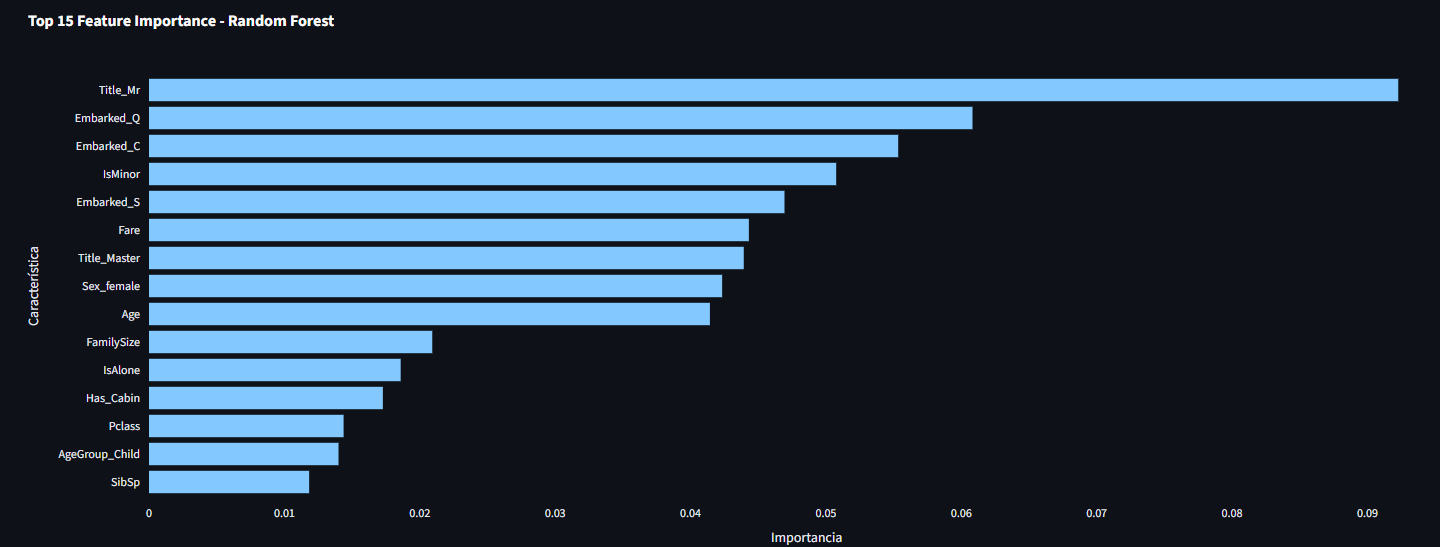
\includegraphics[width=\linewidth]{figures/FeatureImportanceRandomForestDashboard.png}
    \caption{Feature Importance - Random Forest (Dashboard)}
    \label{fig:placeholder}
\end{figure}

\section{Consideraciones Éticas Extendidas}
\subsection*{Identificación de Stakeholders}
Los principales actores involucrados en el análisis y aplicación de modelos predictivos sobre el Titanic incluyen:
\begin{itemize}
    \item Pasajeros y tripulación representados en los datos, cuyo registro apoya al trabajo y los resultados del mismo.
    \item La comunidad académica y de ciencia de datos, que utilizará este trabajo, modelo y análisis resultante como punto de referencia para futuros trabajos y/o aportaciones.
    \item Desarrolladores y responsables de sistemas modernos de IA en áreas críticas, quienes pueden extraer reflexiones, análisis y lecciones sobre los modelos siguientes.
\end{itemize}

\subsection*{Escenarios de Posible Uso Indebido}
\begin{itemize}
    \item Trivializar o minimizar tragedias humanas al reducirlas únicamente a métricas de predicción.
    \item Utilizar modelos entrenados con sesgos históricos para justificar decisiones actuales sin un análisis crítico.
    \item Aplicar técnicas de interpretabilidad de forma aislada, sin considerar las dimensiones éticas y sociales de los datos.
\end{itemize}

\subsection*{Estrategias y Mitigaciones Propuestas}
\begin{itemize}
    \item Mantener siempre la dimensión humana en el análisis: los datos representan vidas y desigualdades reales que pasaron, no son solo estadísticas.
    \item Priorizar métricas que reduzcan la exclusión de posibles sobrevivientes (Por ejemplo: Recall) frente a métricas de precisión exclusivamente técnicas.
    \item Incorporar revisiones interesccionales (género x clase x edad) y auditorías de fairness con métricas múltiples (paridad demográfica, igualdad de oportunidades, etc).
    \item Utilizar el caso del Titanic como un ejemplo ilustrativo para reflexionar sobre cómo los sesgos históricos pueden repetirse en aplicaciones modernas, contribuyendo con un análisis crítico y evitando generalizaciones sin análisis.

\end{itemize}

\end{document}

